\newcommand{\bx}{{\bf x}}
\newcommand{\bl}{\boldsymbol{\ell}}
\newcommand{\fts}{{\widetilde{s}}}
\newcommand{\ftr}{{\widetilde{r}}}
\newcommand{\ftv}{{\widetilde{v}}}
\newcommand{\bu}{{\bf u}}
\newcommand{\bb}{{\bf b}}
\newcommand{\ftR}{{\widetilde{R}}}

\documentclass[twocolumn]{emulateapj}
\usepackage{amsmath}
\usepackage{graphicx}
\usepackage{natbib}
\usepackage{color}
\usepackage{hyperref}
\citestyle{aa}


\begin{document}
\title{The Hydrogen Epoch of Reionization Array Dish II: Characterization of Spectral Structure with Electromagnetic Simulations and their Science Implications}
\author{
Ewall-Wice Aaron\altaffilmark{1,2},
Richard Bradley\altaffilmark{3,4},
Abraham Neben\altaffilmark{1,2},
Nipanjana Patra\altaffilmark{5},
Nithyanandan Thyagarajan \altaffilmark{6},
Jacqueline Hewitt\altaffilmark{1,2},
Zaki S. Ali\altaffilmark{5},
Judd Bowman\altaffilmark{6},
Carina Cheng\altaffilmark{5},
David Deboer\altaffilmark{5},
Aaron Parsons\altaffilmark{5},
Mariet Venter\altaffilmark{7}
and others.
}

\altaffiltext{1}{MIT Kavli Institute for Cosmological Physics}
\altaffiltext{2}{MIT Dept. of Physics}
\altaffiltext{3}{National Radio Astronomy Obs., Charlottesville VA}
\altaffiltext{4}{Dept. of Astronomy, U. Virginia, Charlottesville VA}
\altaffiltext{5}{Astronomy Dept. U. California, Berkeley CA}
\altaffiltext{6}{School of Earth and Space Exploration, Arizona State U.,
\altaffiltext{7}{Stellenbosh}
Tempe AZ}
\begin{abstract}
We use time domain electromagnetic simulations to assess the spectral characteristics of the antenna element for the Hydrogen Epoch of Reionization Array (HERA). These simulations are part of a multi-faceted campaign to determine whether the dish's design is suitable for obtaining a detection of redshifted 21\,cm emission from the Epoch of Reionization. Our simulations show the existence of standing wave reflections in some regions of the 100-200\,MHz bandpass with an amplitude of $\approx -35$\,dB at 100\,ns which can lead to some loss of measurable modes and a modest reduction in sensitivity over a small segment of the band. Overall, we find that the spectral response of the dish is sufficiently smooth for proven foreground isolation methods such as delay filtering to contain foreground emission at line of sight wave numbers below $k_\parallel = 0.15-0.2$\,$h$Mpc$^{-1}$. Incorporating these results into a Fisher Matrix analysis, we find that the spectral structure observed in our simulations has only a small effect on the overall constraints on the astrophysics of reionization that HERA will achieve, allowing it to serve as a benchmark for the design of future instruments such as the Square Kilometer Array. 
\end{abstract}
\section{Introduction}
Observations of the redshift 21\,cm radiation neutral hydrogen in the intergalactic medium (IGM) have the potential to illuminate the hitherto unobserved {\it dark ages} and {\it cosmic dawn}, revolutionizing our understanding of the first UV and X-ray sources in the universe and how their properties influenced galactic evolution (see \citet{Furlanetto:2006Review}, \citet{Morales:2010}, and \citet{Pritchard:2012} for reviews). As of now, two major experimental endeavors are underway to make a first detection of the 21\,cm signal with most focusing on the Epoch of Reionization (EoR) in which UV photons from early galaxies transformed the hydrogen in the universe from neutral to ionized. The first involves measuring the sky-averaged global signal and is being pursued by experiments such as EDGES \citep{Bowman:2010}, LEDA \citep{Greenhill:2012,Bernardi:2015}, DARE \citep{Burns:2012}, SciHi \citep{Voytek:2014}, and BIGHORNS \citep{Sokolowski:2015} either in their planning stages or already taking data. The second attempts to observe spatial  fluctuations in the 21\,cm emission using radio interferometers. A first generation of such experiments are currently taking data in an attempt to make a first statistical detection of the power spectrum of 21\,cm brightness temperature fluctuations. These include the Giant Metrewave Telescope (GMRT)  \citep{Paciga:2013}, the Low Frequency ARray (LOFAR), \citep{VanHaarlem:2013}, the Murchison Widefield Array \citep{Tingay:2013a} and the Precision Array for Probing the Epoch of Reionization (PAPER) \citep{Parsons:2010}. Already, these experiments are beginning to yield upper limits on the 21\,cm signal \citep{Dillon:2013,Parsons:2014,Jacobs:2015,Dillon:2015,EwallWice:2015a} and significant scientific results. The most stringent measurement of $\approx 500$\,mK$^2$ \citep{Ali:2015} is able to rule out number of scenarios in which the intergalactic medium received little or no heating from X-rays \citep{Pober:2015,Greig:2015b}. 

The primary obstacle to obtaining a high redshift detection of the cosmological signal through both of these methods is the existence of foregrounds that are $\sim 10^5-10^6$ times brighter. While requiring much greater sensitivity than global-signal experiments, interferometers have the advantage that spectrally smooth foregrounds are naturally contained to a finite region of Fourier space, corresponding to large line of sight scales, known as the {\it wedge} \citep{Datta:2010,Vedantham:2012,Parsons:2012,Thyagarajan:2013,Liu:2014a,Liu:2014b}. However any structure in the frequency response of the instrument is imprinted on the foregrounds and has the potential to leak power into the {\it EoR window} at small line of sight scales, masking the signal. Indeed, sub-percent spectral features in the analogue and digital signal chains on the initial build-out of the MWA are proving to be a significant obstacle \citep{Dillon:2015b,EwallWice:2015a,Beardsley:2015b}. 

While, in principle, spectral structure in the bandpass of the instrument may be removed in calibration, simulations show that any mismodeling of emission and the primary beam, potentially below the confusion limit, will mix the significant spectral structure introduced by the wedge on long baselines into short ones, masking the signal entirely \citep{Barry:2016}. While redundant calibration \citep{Wieringa:1992,Liu:2011,Zheng:2014} is able to solve for gains that are primarily independent of a detailed model of the sky, it is unclear how one might remove direction-dependent chromatic structure that might be present in the primary beam of the instrument. Because of our limited knowledge of foregrounds at low frequency and the fidelity of calibration algorithms, it is imperitive to design experiments whose spectral structure is contained, as much as possible, to low delays. 

The Hydrogen Epoch of Reionization Array (HERA) is a next generation 21\,cm experiment designed to achieve a two-orders of magnitude improvement in sensitivity over current experiments which will allow it to make a robust detection of the 21\,cm power spectrum during the EoR \citep{Pober:2014}. Much of this sensitivity increase is enabled by moving the collecting area of the instrument into baselines that are located primarily inside of the EoR window and a switch from PAPER's skirted dipoles and the MWA's phased dipole arrays to an antenna element that consists of a feed suspended over a large reflecting parabolic dish. A central requirement for HERA's dish design is that the antenna have a response that is sufficiently smooth in frequency and centralized enough in its angular response that it leaves the EoR window free of contamination since one cannot rely on direction independent redundant calibration to remove any spectral structure that varies as a function of location on the primary beam. 

This paper and its companions \citep{Neben:2016,Patra:2016,Thyagarajan:2016} describe a multifaceted approach for assessing whether the HERA dish meets the requirements for isolating foregrounds within the wedge and leaving the EoR window clean. We accomplish this by establishing a spec with simulations of foregrounds \citep{Thyagarajan:2016} and verifying that HERA primary antenna element meets this spec with reflectometry \citep{Patra:2016} and Orbcomm beam mapping \citep{Neben:2016}. In this work, we present the results of time-domain electromagnetic simulations that are intended to predict the degree of spectral structure in the HERA dish, assess the impact of this spectral structure on the leakage of foregrounds into the EoR window, and to verify the reflectometry measurements taken in the field by \cite{Patra:2016}. 

This paper is organized as follows. In \S~\ref{sec:Formalism} we lay out our analytic framework and describe the impact of reflections and spectral structure on foreground leakage in delay-transform power spectra. In \S~\ref{sec:Simulations} we describe our time-domain electromagnetic simulations of the HERA dish element and how we extract the voltage response function. In \S~\ref{sec:SimulationResults} we describe the results and verify our simulation framework by comparing its prediction of the $S_{11}$ parameter of the HERA dish to direct field measurements described in \citep{Patra:2016}. In \S~\ref{sec:Foregrounds} we apply our electromagnetic simulation results to simulations of foregrounds to determine the extent that the HERA dish's chromatic structure pollutes the EoR window and their impact on HERA's overall sensitivity. We conclude in \S~\ref{sec:Conclusion}.

\section{The Impact of Reflections on Delay-Transform Power Spectra}\label{sec:Formalism}
In this section, we show how reflections in the analogue signal path of an antenna lead to foreground contamination of the EoR window. Intuitively, any reflections in the signal path introduce sinusoidal ripples in the frequency dependent gain of the instrument. Since time delay is the Fourier dual to frequency, reflections with larger delays introduce ripples at higher frequencies. Isolation of the 21\,cm signal from foregrounds that are over five orders of magnitude brighter depends critically on their smoothness. Any sinusoidal frequency structure introduced by the reflections will cause these foregrounds to mimic and swamp the signal unless they are brought below a level similar to the ratio between the foregrounds and the signal itself. A simple equation describing effect of direction independent reflections in the signal chain of an interferometer, downstream of the receiver on a visibility has been derived in \citet{EwallWice:2015a}. We now extend this analysis by considering the direction dependent reflections that can occur within the antenna element. 
We start by denoting the electric field of radiation arriving at an $i^{th}$ antenna element at position $\bx_i$ and time $t_i = t + \bl \cdot \bx_i /c \equiv t+\tau_i$ as $\fts(\bl,\bx_i,t_i)$. 

Reflections within the signal chain of each antenna are most generally described by a direction dependent reflection coefficient, $\ftr_i(\bl,\tau)$. Its effect is to add the signal to itself multiplied by $\ftr_i$ and delayed by $\tau$. The voltage signal measured at the $i^{th}$ antenna element, $\widetilde{v}_i$, is the integral over solid angle of the electric fields arriving from all directions. The presence of the reflections introduces a convolution of the electric field entering the antenna (delayed by $\tau_i$) with $\ftr_i(\bl,\tau)$.

\begin{equation}\label{eq:Voltage}
\ftv_i(t) = \int d \Omega \int d \tau \ftr_i(\bl,\tau) \fts(\bl,t+ \tau_i - \tau)
\end{equation}

A correlator measures the time-averaged product of the Fourier transform of the voltage streams between the $i^{th}$ and $j^{th}$ antenna. Fourier transforming the voltage stream from the $i^{th}$ antenna we obtain
\begin{equation}
v_i(f) = \int d \Omega \int d \tau \ftr_i(\bl,\tau) s(\bl,f)e^{-2 \pi i f(\tau_i+\tau)}
\end{equation}
The time averaged product between the two antennas is
\begin{align}
V_{ij}'(f) &= \left \langle v_i(f) v_j^*(f) \right \rangle_t \nonumber \\
 &= \int d \Omega d \tau d \tau' \ftr_i(\tau) \ftr^*_j(\tau')e^{-2 \pi i f (\tau-\tau') } I(\bl, f) e^{- 2 \pi i \Delta \tau_{ij}f} 
\end{align}
where $\Delta \tau_{ij} = \tau_i-\tau_j = (\bx_i-\bx_j) \cdot \bl/c$ and $I(\bl,f)=\left \langle |s(f,\bl)|^2 \right \rangle_t$. Here, we have invoked the fact that electromagnetic waves arriving from different directions are incoherent. 

Defining $\bu_{ij} = f (\bx_i-\bx_j)/c$ and performing the $\tau$ and $\tau'$ Fourier transforms, we arrive at
\begin{equation}\label{eq:Visibility}
V'_{ij}(f) =  \int d \Omega r_i(\bl,f) r^*_j(\bl,f)  I(\bl,f)e^{2 \pi i f \bu_{ij} \cdot \bl/c},
\end{equation}
where ${\bf b}_{ij} = ({\bf x}_i - {\bf x}_j )$ to use the usual $uv$ notation of interferometry. $r_i(\bl,f)$ is the inverse fourier transform of the reflection response of the dish, hence we see that the reflection response is precisely the Fourier dual to the Dish's frequency domain voltage beam. Setting a specification on reflections is hence equivalent to setting a specification on the spectral smoothness of the antenna's voltage beam. 

In order to filter spectrally smooth foregrounds from the signal,HERA is expected to employ the {\it delay transform} over frequency, defined as \citep{Parsons:2012}
\begin{equation}
\widetilde{V}_{ij}(\tau) = \int d f e^{2 \pi i \tau f} V_{ij}(f).
\end{equation}
Applying this to equation~\ref{eq:Visibility}, we obtain
\begin{equation}
\widetilde{V}'_{ij}(\tau)=  \int d \Omega \int d f  r_i(\bl,f) r_j^*(\bl,f)  I(\bl,f) e^{2 \pi i f ( \bb_{ij} \cdot \bl /c - \tau)}
\end{equation}
Let's examine the quantity within the angular integral. We see that each source located at $\bl$ on the sky is mapped to a line $\tau =\bb_{ij}\cdot \bl/c$, resulting in the much discussed ``wedge" \citep{Datta:2010,Vedantham:2012,Parsons:2012,Morales:2012,Thyagarajan:2013,Liu:2014a,Liu:2014b}. The presence of the frequency dependent beam causes each source line to be convolved in delay with the direction dependent kernel
\begin{equation}\label{eq:Kernel}
\ftR_{ij}(\bl,\tau) = \int d \tau \ftr_i(\bl,\tau - \Delta \tau) \ftr^*_j(\bl,-\Delta \tau).
\end{equation}
which is the convolution of the delay response of the voltage beam of antenna $i$ with the time-reversed complex conjugate of voltage beam of antenna $j$. In the remainder of this paper, we will often refer to $\ftR$ as the {\it power kernel} applied to a visibility. Note that this is not equal to the convolution of the voltage response with its complex conjugate, which would lead to foreground power only being bled out to positive delays. We demonstrate the effect of foreground smearing in Fig.~\ref{fig:Smearing} for a simple model with only three sources. Without reflections, the sources would form lines in $b-\tau$ space. Withthe reflections, the sources are smeared out, leading to supra-horizon emission. 
\begin{figure*}
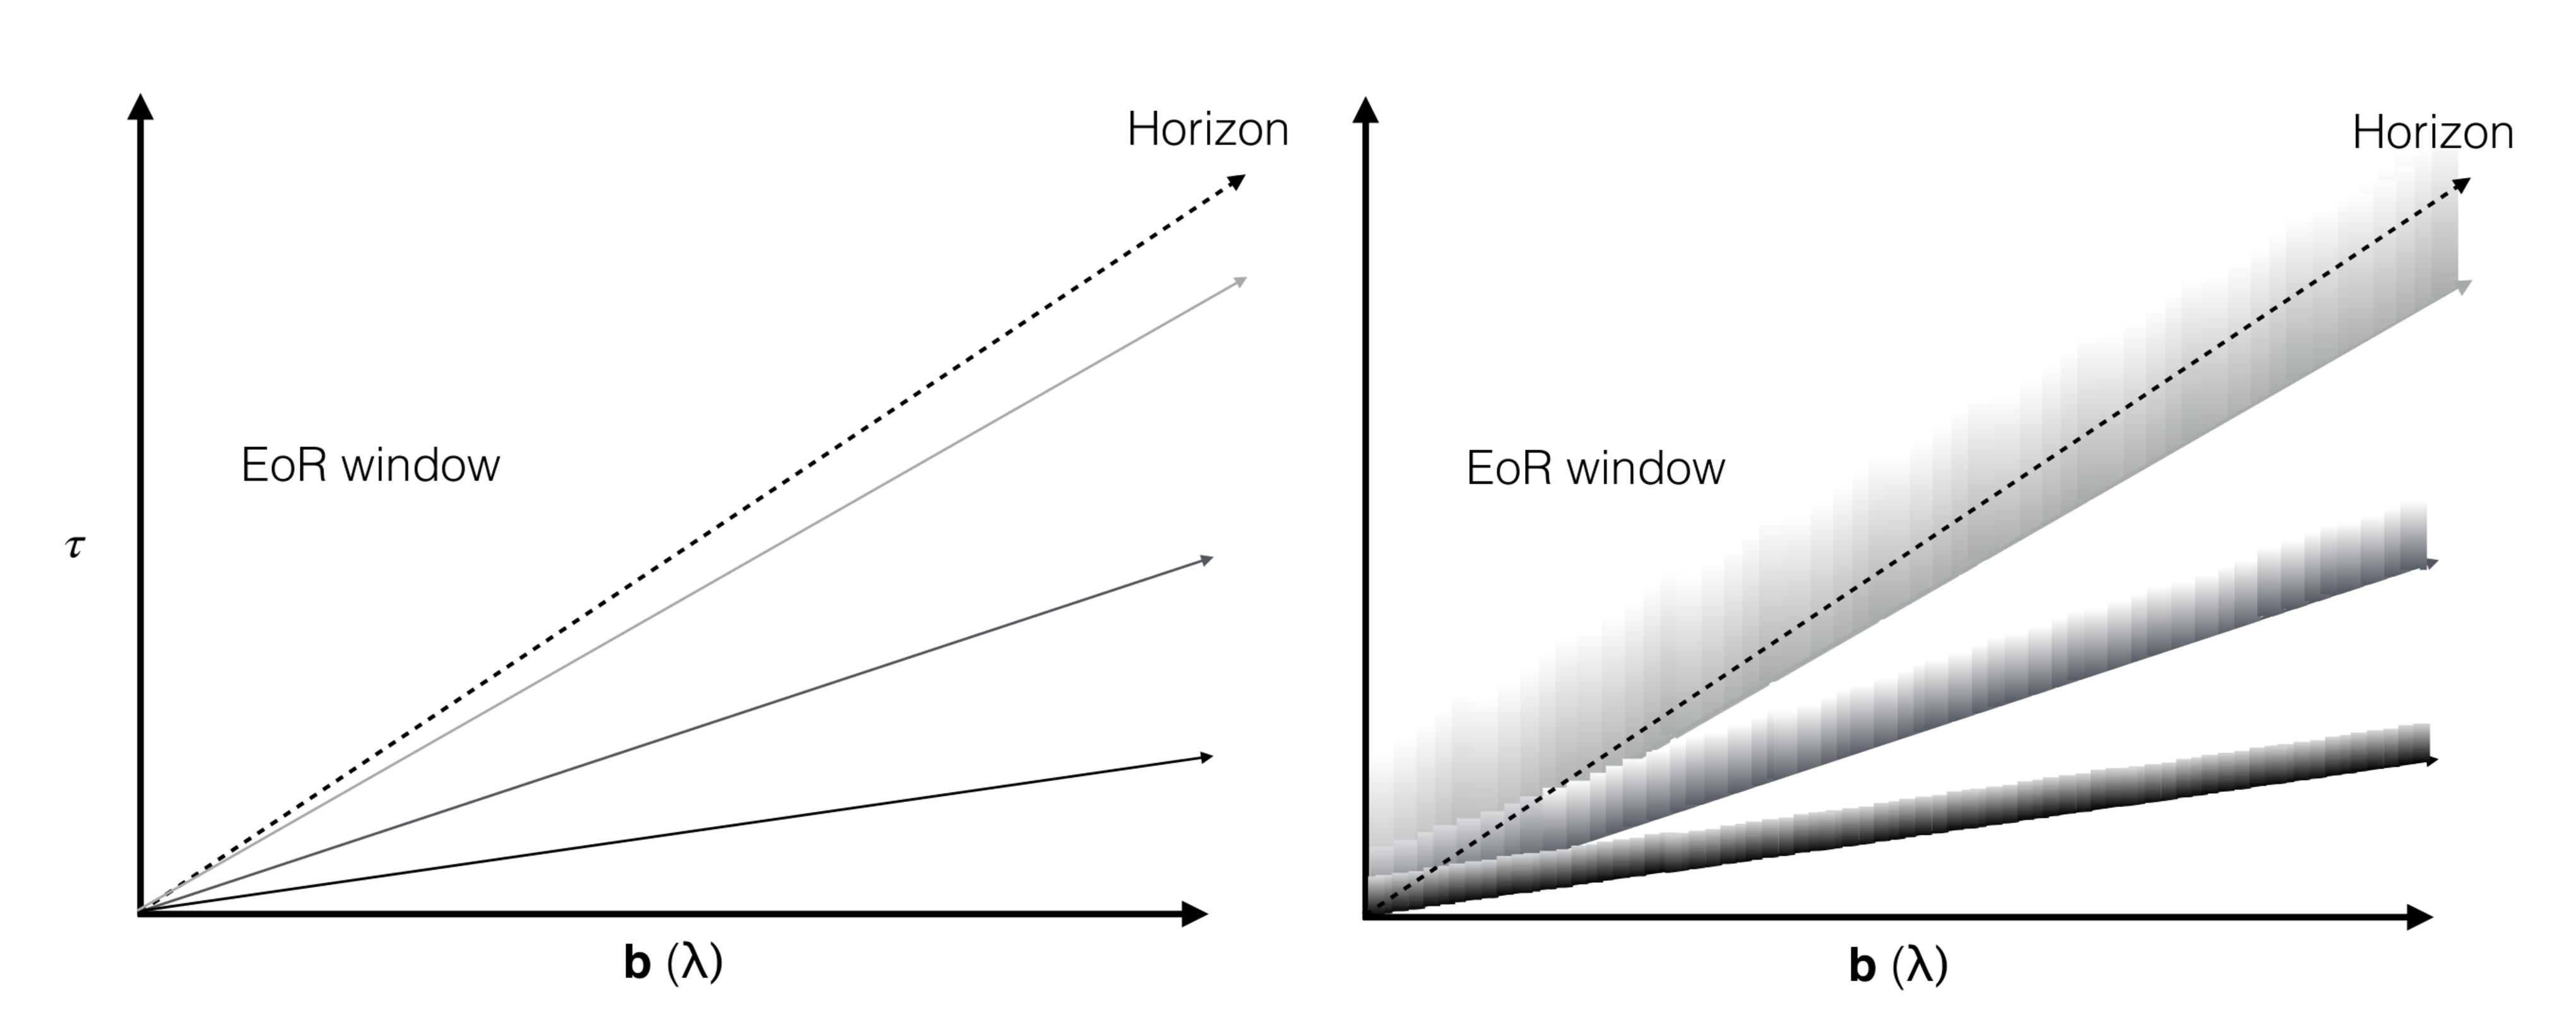
\includegraphics[width=\textwidth]{figures/wedgeCompare.pdf}
\caption{A demonstration of the impact on foregrounds of the frequency dependent beam. Left: The location of three sources in delay space assuming a frequency indepdendent beam (no reflections in the antenna element). Right: the presence of chromaticity due to reflections in the antenna smears the source in delay with the kernel given by equation~\ref{eq:Kernel}. Since the frequency response of the dish are a function of direction on the sky, the shape of the delay kernel is different for each source line. We see that this smearing can lead to substantial supra-horizon emission. Sources near zenith (low delay) tend to have a larger maximum since the beam gain is larger near zenith, but a more compact kernel (since beam bore-sights tend to have less spectral structure). Meanwhile, sources near the horizon have a much smaller maxima but have less compact kernels.}
\label{fig:Smearing}
\end{figure*}
For the sake of pedagogy, we now consider the case where the beam can be factored into angular and frequency independent components, $r_i(\bl,f) = g_i(f)a_i(\bl)$. For such a case, every line in Fig.~\ref{fig:Smearing} would be convolved with the same delay dependent shape, normalized to the gain of $a_i(\bl)$. In this situation, we have
\begin{equation}
\widetilde{V}_{ij}'(\tau) = \int d\tau' \int d \tau'' \widetilde{g}_i(\tau' - \tau'')\widetilde{g}^*_j(\tau'') \widetilde{V}_{ij}(\tau-\tau')
\end{equation}
where $V_{ij}$ is the visibility with the achromatic factor in the voltage patterns included. 
We can gain further insight into the behavior of the delay kernel arising from chromaticity by assuming that $\widetilde{g}_i(\tau=0)\gg\widetilde{g}_i(\tau>0)$, which should be the case at large delays for the smooth bandpasses our instruments are designed to have. 
\begin{align}\label{eq:KernelApprox}
\widetilde{V}_{ij}'(\tau) &\approx \widetilde{g}_i(0)\int d \tau' \widetilde{g}_j^*(\tau')\widetilde{V}_{ij}(\tau- \tau') \nonumber \\
& + \widetilde{g}_j^*(0) \int d \tau' \widetilde{g}_i(\tau')\widetilde{V}_{ij}(\tau-\tau') 
\end{align}
Hence, to first order, the impact of reflections is to convolve the delay-transformed visibility with the voltage beam of the instrument. This may be a somewhat un-intuitive result since naive dimensional analysis might predict that the power-kernel to be proportional to the square of the delay-response. This linear falloff coupled with the enormous dynamic range between foregrounds and signal puts exquisite requirements on the smoothness of the beam, requiring that it fall roughly six orders of magnitude in the regions of delay space that we want to measure the signal.


\section{Electromagnetic Simulations of the HERA dish element}\label{sec:Simulations}

HERA \citep{DeBoer:2016} is an instrument designed to detect the power spectrum of 21\,cm brightness temperature fluctuations during the EoR at high signal-to-noise between the frequencies of 100 and 200\,MHz (redshifts 6 to 12) \citep{Pober:2014}. Its initial, 19-element, buildout is currently taking first observations in the Karoo in South Africa. HERA is meant to serve as a vast improvement in sensitivity over current efforts for only a modest increase in cost. It achieves this by increasing the number of correlated inputs by only a factor of $\approx 2$ while increasing the total collecting area of each correlated element by over an order of magnitude and arranging the elements in such a way as to maximize the number of short baselines that are located outside of the foreground wedge. Central to increasing the collecting area of each element is a switch from dipoles (used by the MWA and PAPER) to feeds suspended over large 14\,m diameter parabolic dishes. In Fig.~\ref{fig:AntennaComparison} we show one of the initial 19 dishes currently being deployed in South Africa at the same site as PAPER whose antenna we also show at the top of the figure. 

Having formally derived the impact of analogue reflections on foreground visibilities, we are now in a position to investigate their existence in the HERA dish. In this section, we describe the setup and parameters of our simulations (\S~\ref{ssec:Simulations}), and how we extract the voltage response function of the dish (\S~\ref{ssec:Deconvolve}).


\begin{figure}
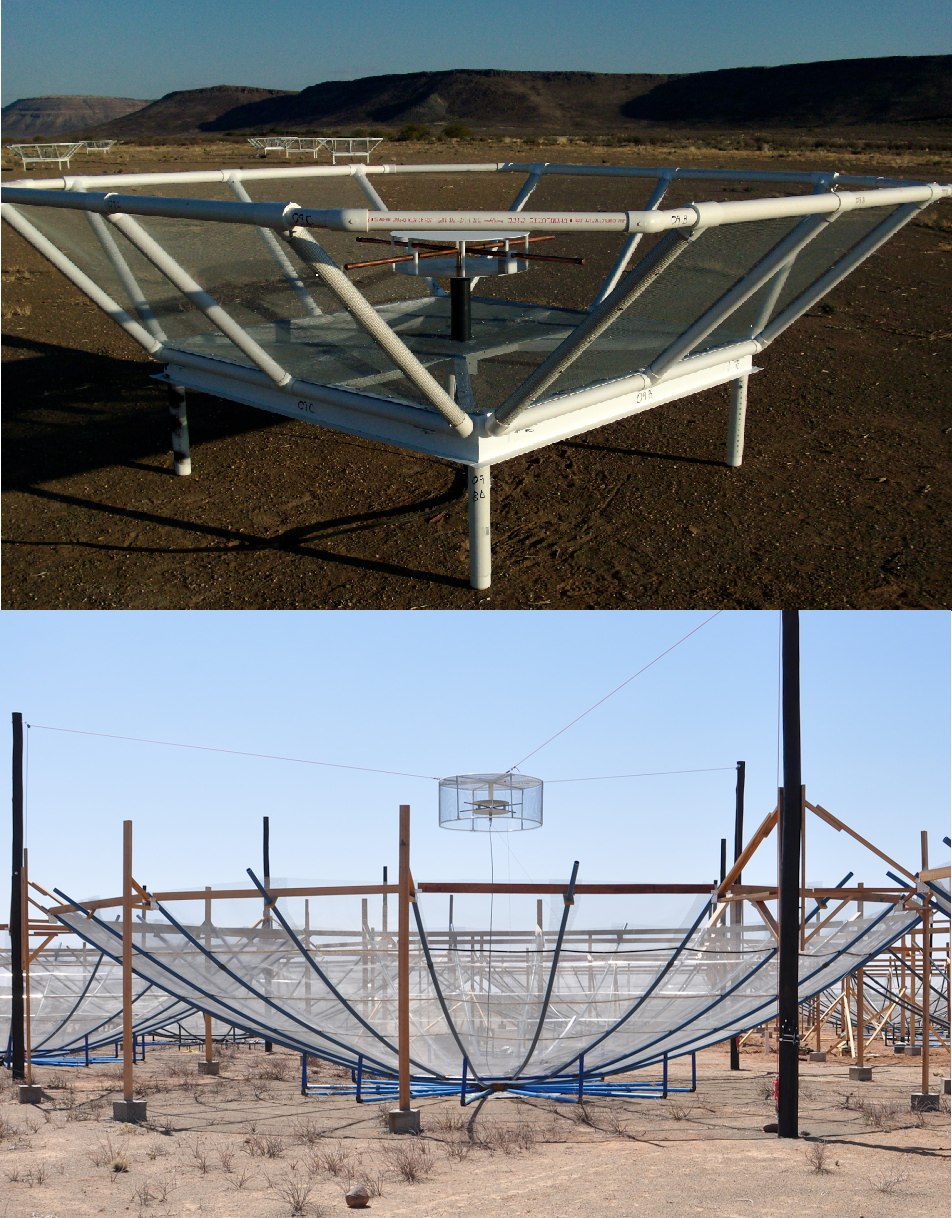
\includegraphics[width=.5\textwidth]{figures/PAPER_HERA_compare.jpg}
\caption{The HERA antenna element (bottom) uses a parabolic dish to achieves over an order of magnitude increase in collecting area over the PAPER antenna (top). The sleeved dipole in the center of the PAPER backplane is identical to the sleeved dipole being suspended under the cylindrical skirt over the vertex of the HERA dish. The dish geometry has the potential to introduce intra-antenna reflections which we explore in this work.}
\label{fig:AntennaCompare}
\end{figure}




\subsection{The Simulations}\label{ssec:Simulations}
We perform time-domain simulations of the voltage output of the HERA feed using CST. {\bf \color{red} Rich: fill in the details here, describe the CST parameters and a brief overview of how it numerically solves for the voltages (citations?).  }

In Fig.~\ref{fig:SimulationSetup} we show the geometery of the electromagnetic simulation. A $150$\,MHz plane wave with a Gaussian envelope with FWHM of {\bf \color{red}???} is initialized {\bf \color{red} ??} meters above the dish vertex traveling in the $-z$ direction. It is reflected by the dish before entering the dipole feed, hidden below the cylindrical skirt in this figure. We record the electric field voltage of the plane wave at the feed output terminals as a function of time, plotted as a red line in Fig.~\ref{fig:SimulationOutput} along with the voltage at the feed outputs (black line). The delay between the primary envelopes of the plane wave and the voltage output of the feed is $\approx 30$\,ns which corresponds to the round trip travel time from the feed to the dish vertex and back. However, while the input plane wave, modulated by a gaussian, falls off rapidly and dies off after the first $\approx 20$\,ns after its peak, we see that the voltage output decays far more slowly with delay due to reflections within the dish-feed structure reintroducing the signal at times beyond its initial falloff. We are able to get a qualitative feel for the amplitude of the reflections by inspecting the falloff of the time domain voltage response and see that after $60$\,ns it reachs $\approx -25$\,dB.
\begin{figure}
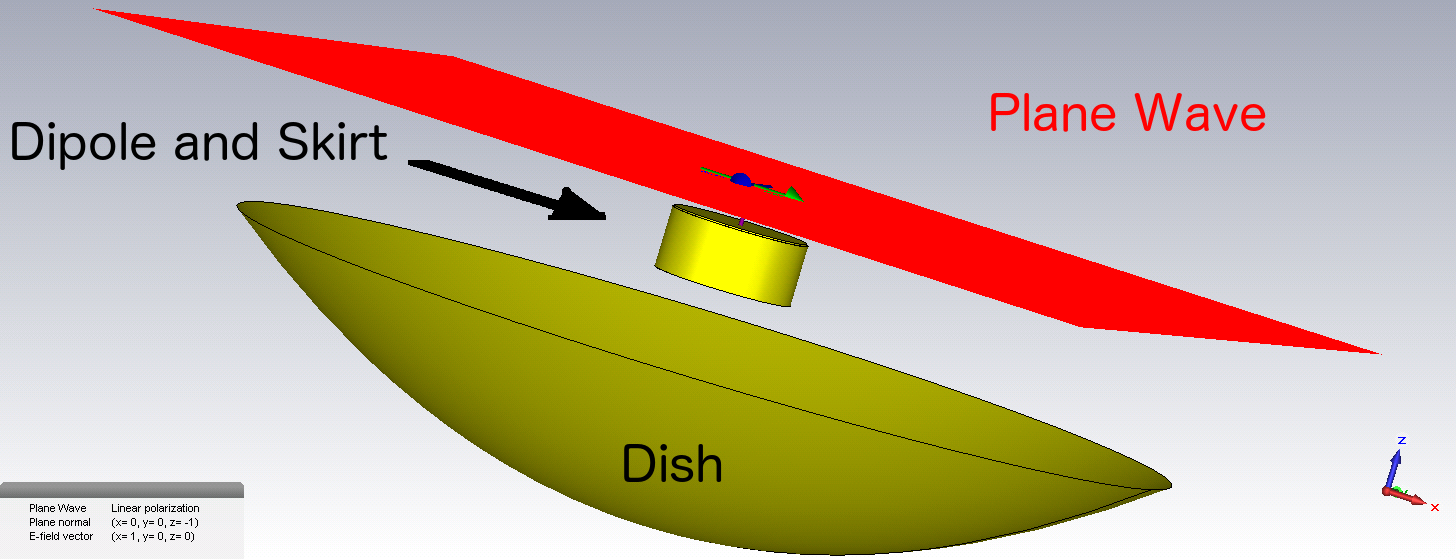
\includegraphics[width=.5\textwidth]{figures/One_dish_Pfeed_render_pw_0deg.png}
\caption{A rendering of our time domain simulation at $t=0$, demonstrating the geometry and setup of our electromagnetic simulation. The plane wave is started just above the feed (red plane).}\label{fig:SimulationSetup}
\end{figure}

\begin{figure*}
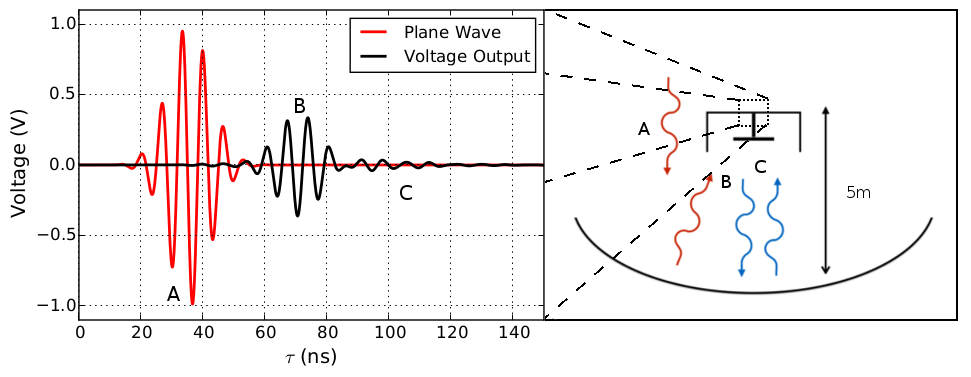
\includegraphics[width=\textwidth]{figures/SimulationIllustration.png}
\caption{An illustration of our simulation products and their origin in the HERA antenna geometry. A plane wave is injected from above the feed (red line). The amplitude of the electric field of the plane wave at output of the feed along with the voltage at the feed terminal outputs is recorded (black line). The feed in our simulation is situated $5$\,m above the bottom of the dish, hence there is a $\approx 30$\,ns delay between when the plane wave passes the terminal for the first time (A) and when it is first absorbed in the dipole (B), leading to the voltage response. Of concern to 21\,cm experiments are the subsequent reflections between the feed and the dish (C) which can lead to large delay contamination of the EoR window.}
\label{fig:SimulationOutput}
\end{figure*}
\subsection{Deconvolving the Response Function}\label{ssec:Deconvolve}

We can do much better than this. From equation~\ref{eq:Voltage}, we know that the voltage output results from the convolution of the plane wave input with the voltage gain of the antenna. The voltage response of the dish which we are attempting to probe has been convolved with a known kernel; our input plane wave. Hence, a straightforward application of the Fourier convolution theorem allows us to determine the voltage response.

Since our simulation is sampled in finite time steps, we will adopt discretized notation for this section. In particular, our simulation consists of $N$ samples, evenly spaced by $d \tau$ at times $\tau_n = n \times d \tau$. 
We denote the output voltage at the feed terminals at time $\tau_n$ as $\widetilde{v}_n$. Rewriting the convolution in equation~\ref{eq:Voltage} in discrete notation, we have
\begin{equation}
\ftv_n({\bf \widehat{k}}) = \sum_m \ftr_m(\bl) \fts_{n-m}(\bl).
\end{equation}
We may undo this convolution by taking a discrete Fourier transform (DFT) of both ${\bf \widetilde{v}}$ and ${\bf \widetilde{s}}$ in time, dividing them in Fourier space, and taking an inverse DFT back. Symbolically,
\begin{equation}\label{eq:Inversion}
\ftr(\bl) = \boldsymbol{\mathcal{F}}^{-1} \left[ \frac{\boldsymbol{\mathcal{F}} {\bf \widetilde{v}}(\bl)}{\boldsymbol{\mathcal{F}}{\fts}(\bl)} \right] 
\end{equation}
where $\boldsymbol{\mathcal{F}}$ is the Fourier transform matrix for a 1d vector of length $N$. 
\begin{equation}
\boldsymbol{\mathcal{F}}_{mn} = e^{2 \pi i m n /N}
\end{equation}
In Fig.~\ref{fig:FrequencyDomain} we show the amplitude of the Fourier transform of our Gaussian input, centered at $150$\,MHz along with the voltage response. Since our input only has support between $\approx 20$ and $280$\,MHz, the direct ratio of our voltage response and input wave is dominated by numerical noise outside of this range. We eliminate these artifacts by multiplying our ratio by a Blackman-Harris window between $100$\,MHz and $200$\,MHz and set our estimate to zero elsewhere. From a physical standpoint, this is sensible since 21\,cm experiments only observe a limited bandwidth. PAPER's correlator, which will initially serve as the HERA backend samples over a $100$\,MHz instantaneous freqeuency interval. Hence analogue filtering is applied to limit the incoming signal within a finite bandwidth and prevent aliasing.

\begin{figure}[h!]
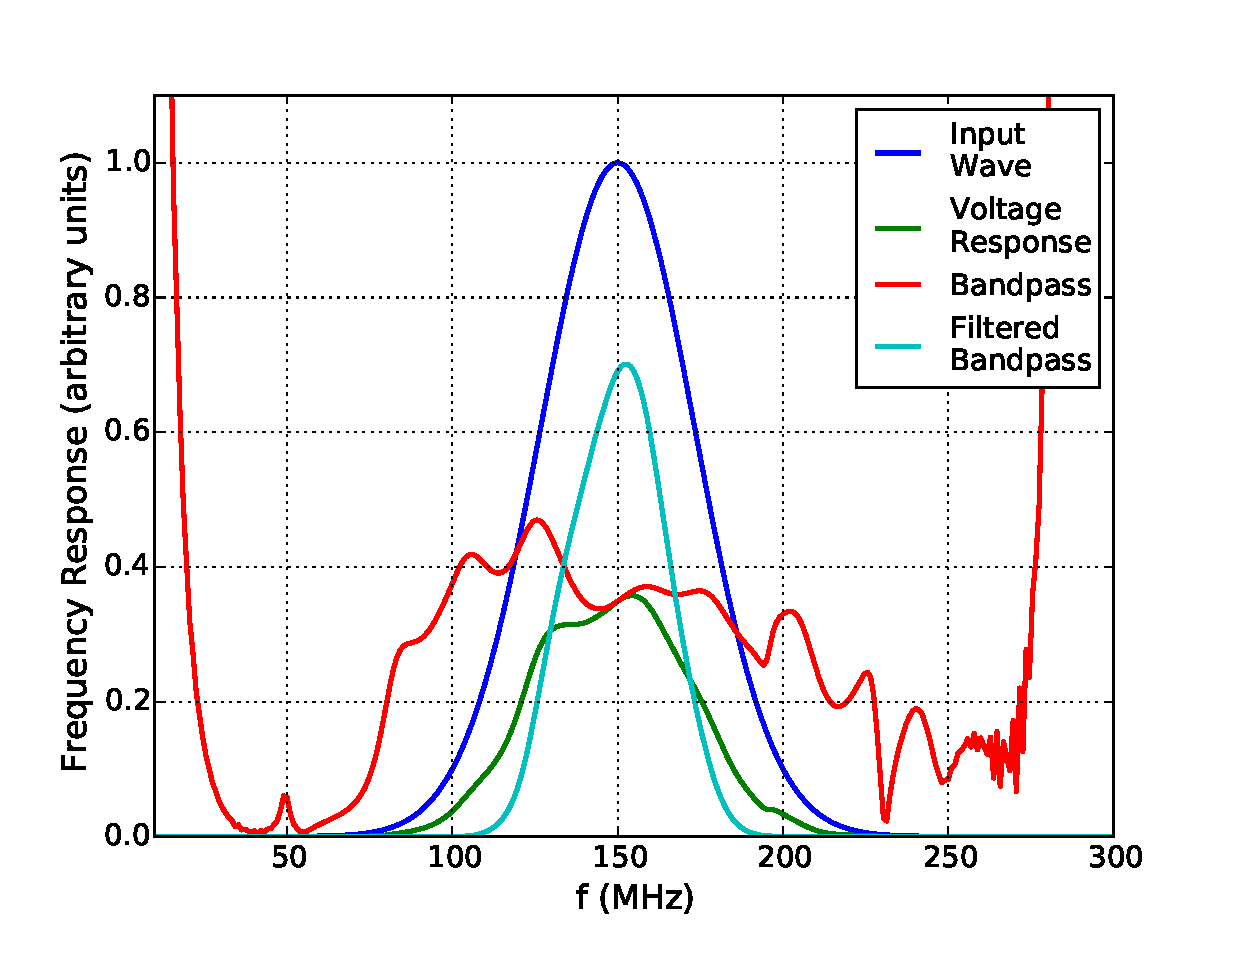
\includegraphics[width=.5\textwidth]{figures/frequency_domain.pdf}
\caption{The absolute value of the discrete Fourier transform of our simulation outputs. We obtain the effective response function of the dish by Fourier transforming the voltage output from our dish (green line) and dividing by the Fourier transform of the input wave (blue line). The simple ratio is plotted as a red line. All lines are normalized to the amplitude of the input wave at $150$\,MHz. Since our input is limited to frequencies between $\approx 20$ and $280$\,MHz, there is significant numerical noise that will effect our result outside of this region which we see in the divergene of the red line towards the edges of the plot. To eliminate this noise, we multiply by a Blackman-Harris window between $100$ and $200$\,MHz and set our estimate to zero elsewhere. The Fourier transform of our response estimate with the filter applied is shown as a cyan line.}
\label{fig:FrequencyDomain}
\end{figure}


\section{Simulation Results}\label{sec:Results}

We now discuss the results of our simulations. In particular, we focus on the time-domain die off of the voltage response and the resulting power kernel (\S~\ref{ssec:Kernel}), comparing it to an identical time-domain simulation of the skirted dipole antenna used by PAPER. In \S~\ref{ssec:Subbands} we investigate the dependence of the power kernel on frequency to determine whether specific parts of the HERA bandpass are more effected than others. Finally, we verify our simulation framework by performing a separate time domain simulation of a measurement of $S_{11}$ of the dish, comparing to a direct field measurement with a vector network analyzer. 

\subsection{The Time Domain Response of the HERA Dish}\label{ssec:Kernel}
Applying equation~\ref{eq:Inversion} to our simulation, we obtain estimates of the time-domain voltage response of the HERA dish towards zenith which we plot in Fig.~\ref{fig:Simulations}. We also conduct a time-domain simulation of the voltage output in response to an identical input plane wave for the skirted dipole PAPER antenna (pictured above the HERA dish in Fig.~\ref{fig:AntennaCompare}) in order to determine whether the presence of the parabolic dish introduces reflections and spectral structure in excess of previous antenna designs for 21\,cm.  We inspect the absolute value of $\ftv$ for both the PAPER and HERA antennas in Fig.~\ref{fig:SimulationResults}. Since non-zero values of $\ftv$ at negative delays violates causality, we assume such features are sourced by numerical artifacts such as side-lobes and/or numerical precision noise which set a limit on the dynamic range of our method. In both the PAPER and HERA simulations, the level of the voltage response at negative delays is on the order of $-60$\,dB. An obvious difference between the two curves is a knee in the HERA gain at $\approx 120$\,ns that is not present in PAPER, leading to a difference in gain of nearly $20$\,dB at 200\,ns. This is an important and perhaps not unsurprising finding: in moving from a skirted dipole to a reflecting dish in order to increase collecting area and overall sensitivity we have added additional chromatic structure. 

Our next step is to compute the power kernel given by      equation~\ref{eq:Kernel}. Since structure at negative delays in our estimate of $\ftv$ is due to numerical artifacts and sidelobes, we set the voltage response to zero at $\tau<0$ before performing a convolution with its time-reverse complex conjugate. In Fig.~\ref{fig:Kernels} we show the power kernel for PAPER and HERA. Since both voltage gains drop rapidly with increasing delay, the approximation in equation~\ref{eq:KernelApprox} holds quiet well and we see that the kernels fall off at a rate similar to the response function itself. 


\begin{figure}[h!]
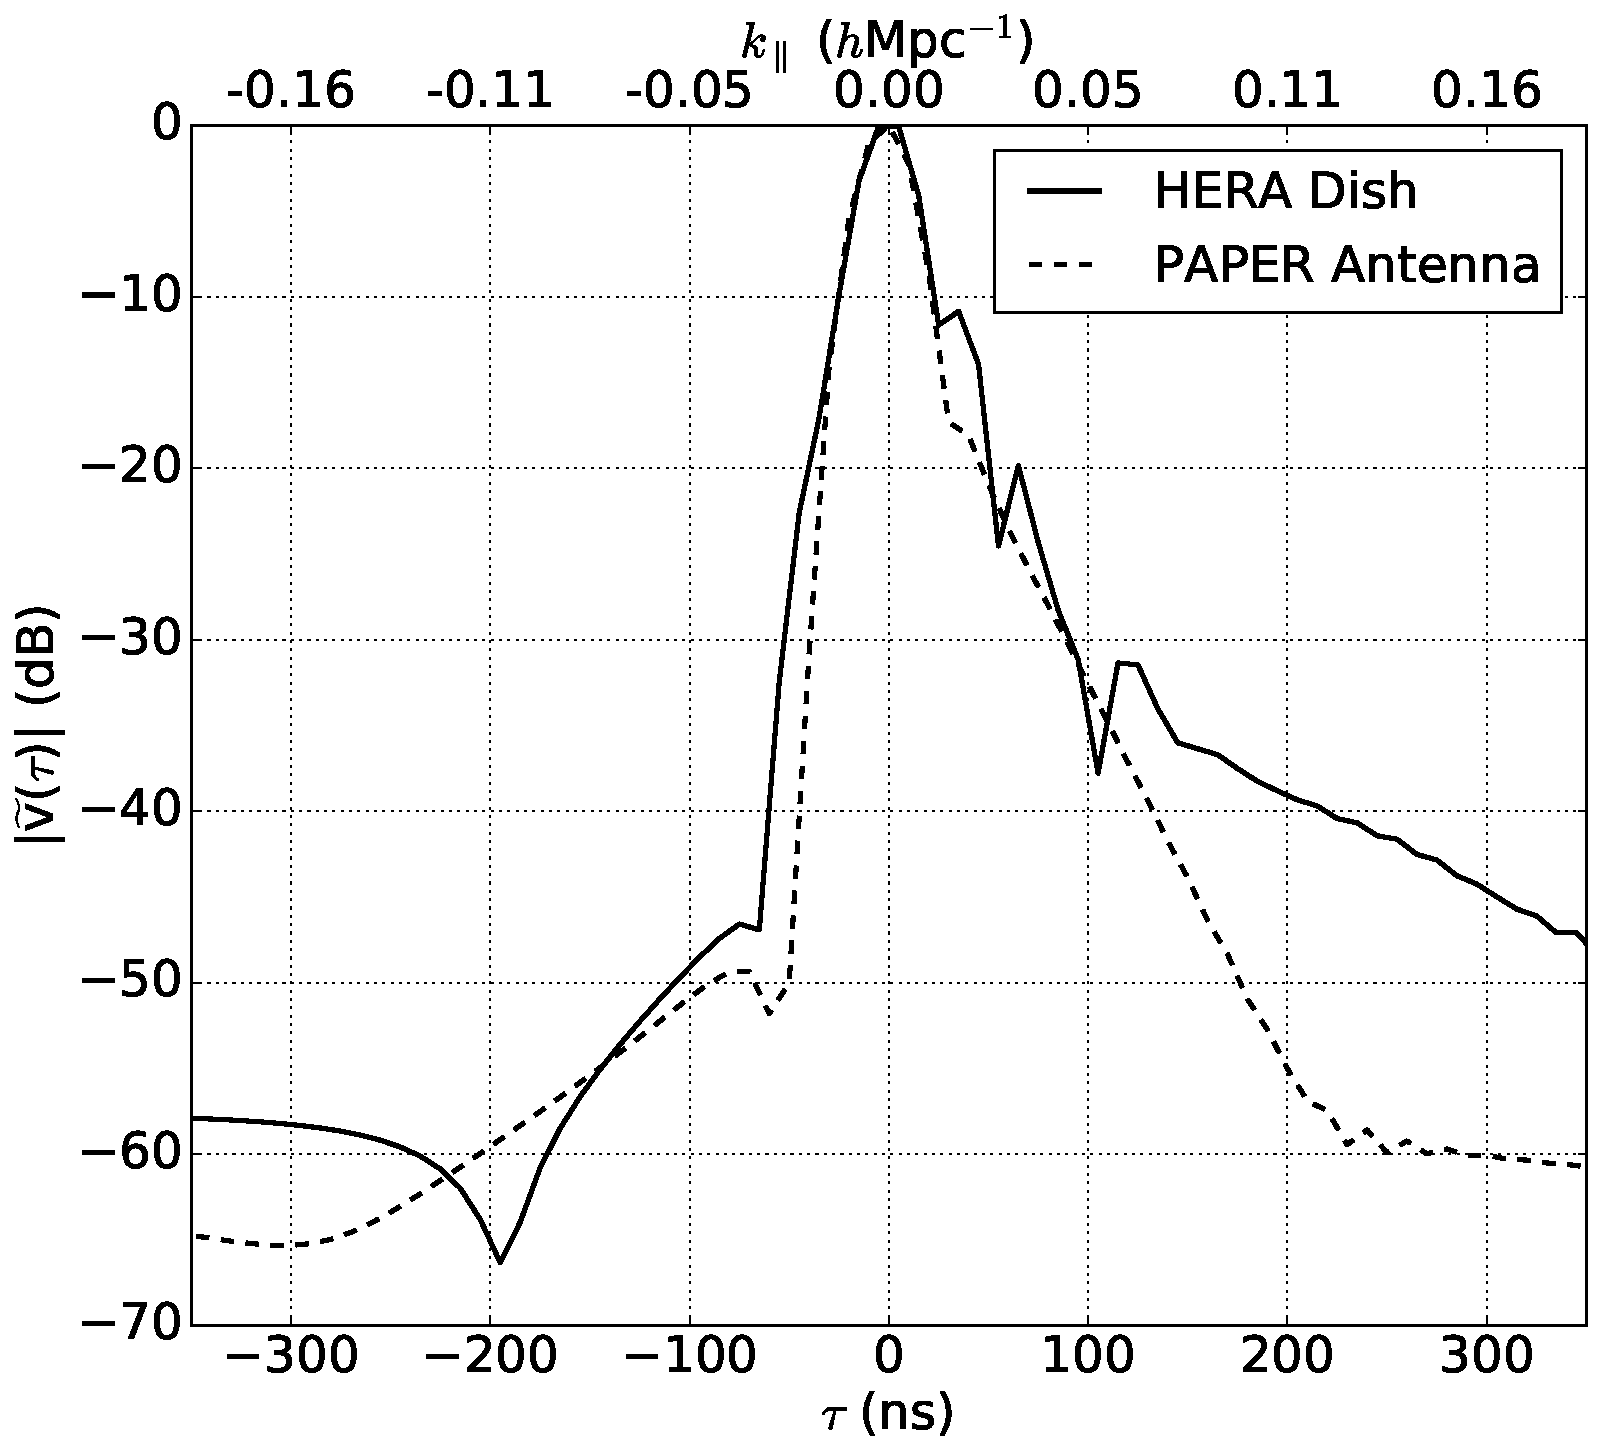
\includegraphics[width=.5\textwidth]{figures/compare_simulations_paper.pdf}
\caption{The Fourier transform of the voltage response function of our simulation for the HERA Dish (solid black line) and the PAPER antenna element (dashed black line). Reflections in the HERA dish element lead to significantly enhanced power above $\sim 50$\,ns. We show the negative delays, which should be devoid of signal, to determine the dynamic range of our technique (which is limited by sidelobes and numerical artifacts). We see that these contaminants exist at the $\sim-60$\,dB level.}
\label{fig:SimulationResults}
\end{figure}



\begin{figure}[h!]
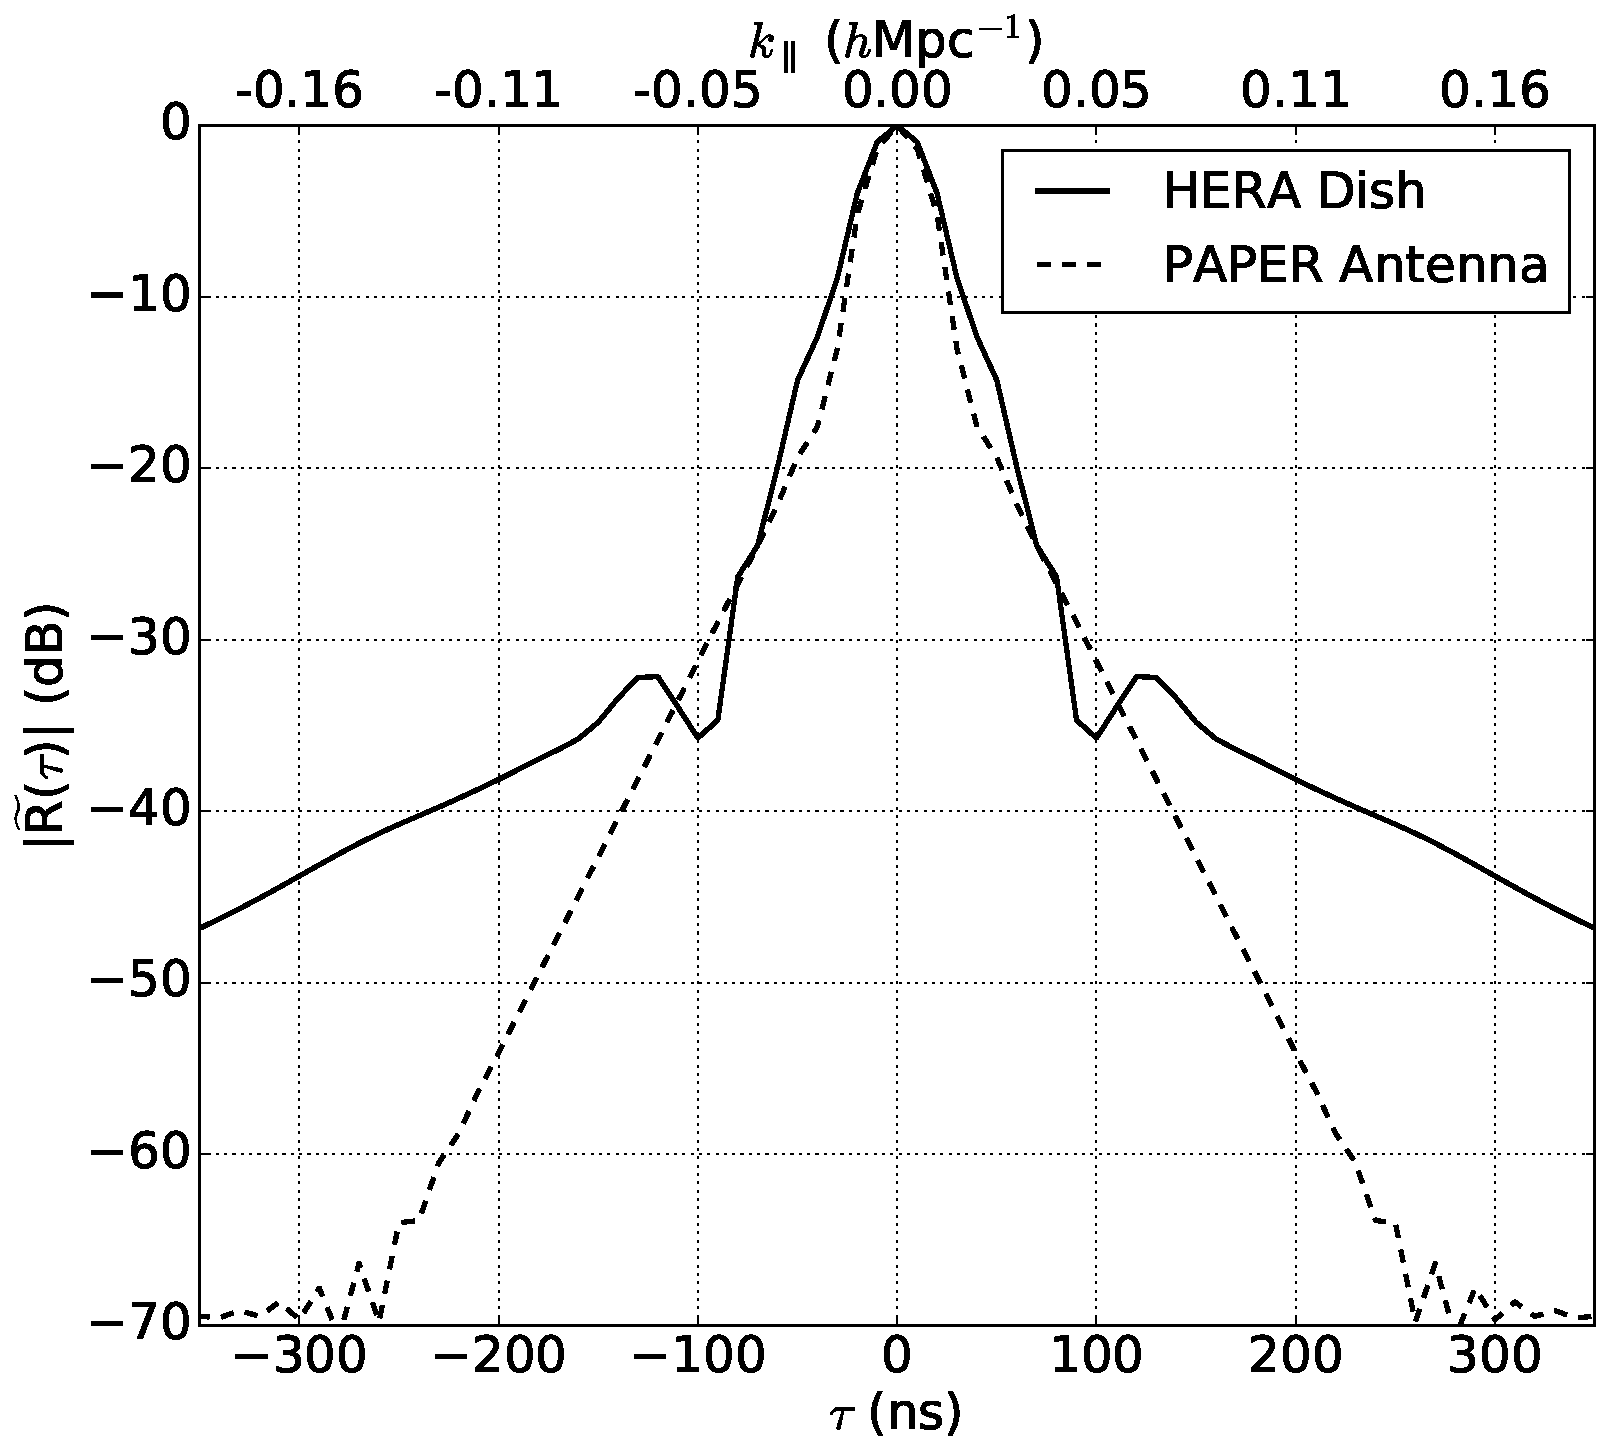
\includegraphics[width=.5\textwidth]{figures/compare_kernels_paper.pdf}
\caption{The absolute value of the power kernel for the HERA dish (solid black line) and for the PAPER antenna element (dashed black line) calculated using equation~\ref{eq:Kernel}. While an antenna can only physically have a voltage response at positive delays, the delay kernel is formed from the convolution of one antenna with the time reversed response function of the other. Hence, the power kernel for two identical antennas will have $\widetilde{R}(\tau) = \widetilde{R}^*(-\tau)$.}
\label{fig:Kernels}
\end{figure}

\subsection{The Delay Response of Subbands}\label{ssec:Subbands}
Because the 21\,cm brightness temperature fluctuations evolve with redshift and follow roughly constant statistics over redshift intervals of $\approx 0.5$ \citep{Zaldarriaga:2004} which corresponds to a bandwidth of $8$\,MHz at $z\approx8$. Thus, how localized the reflections are within the HERA band will also have significant implications. While we observe a long term falloff due to reflections between the feed and dish element, it is possible that these reflections are localized in frequency and do no effect certain sub-bands. To determine whether the reflections are localized in frequency, we compute the voltage delay response and power kernel for three different subbands: $100-130$\,MHz, $130-160$\,MHz, and $160-190$\,MHz. In order to maintain decent resolution of the kernel itself, we use frequency ranges are larger than the actual subbands that will be used for EoR power spectrum estimation $\sim 10$\,MHz. We plot the resulting power kernels in Fig.~\ref{fig:KernelsSubbands}. The central lobe of the delay kernel is significantly wider due to the the wider window functions incurred by the reduced bandwidth. However, the shallow long-term falloff is only visible within the central $125-175$\,MHz band, indicating that long term reflections are isolated near $150$\,MHz and will not effect power spectrum measurements outside of the very center of our band.

To further illustrate the observed isolation of fine frequency structure in the center of the bandpass and to verify that our observations are not an artifact of our reduction of the simulation outputs, we fit the $10$\,MHz intervals of the absolute value of the simulated gains to a sixth order polynomial and compare the residuals in Fig.~\ref{fig:Residuals}. We find that the gain residuals on the sixth order fit are an order of magnitude greater over the $145-155$\,MHz subband than over any other frequency interval. 


\begin{figure}[h!]
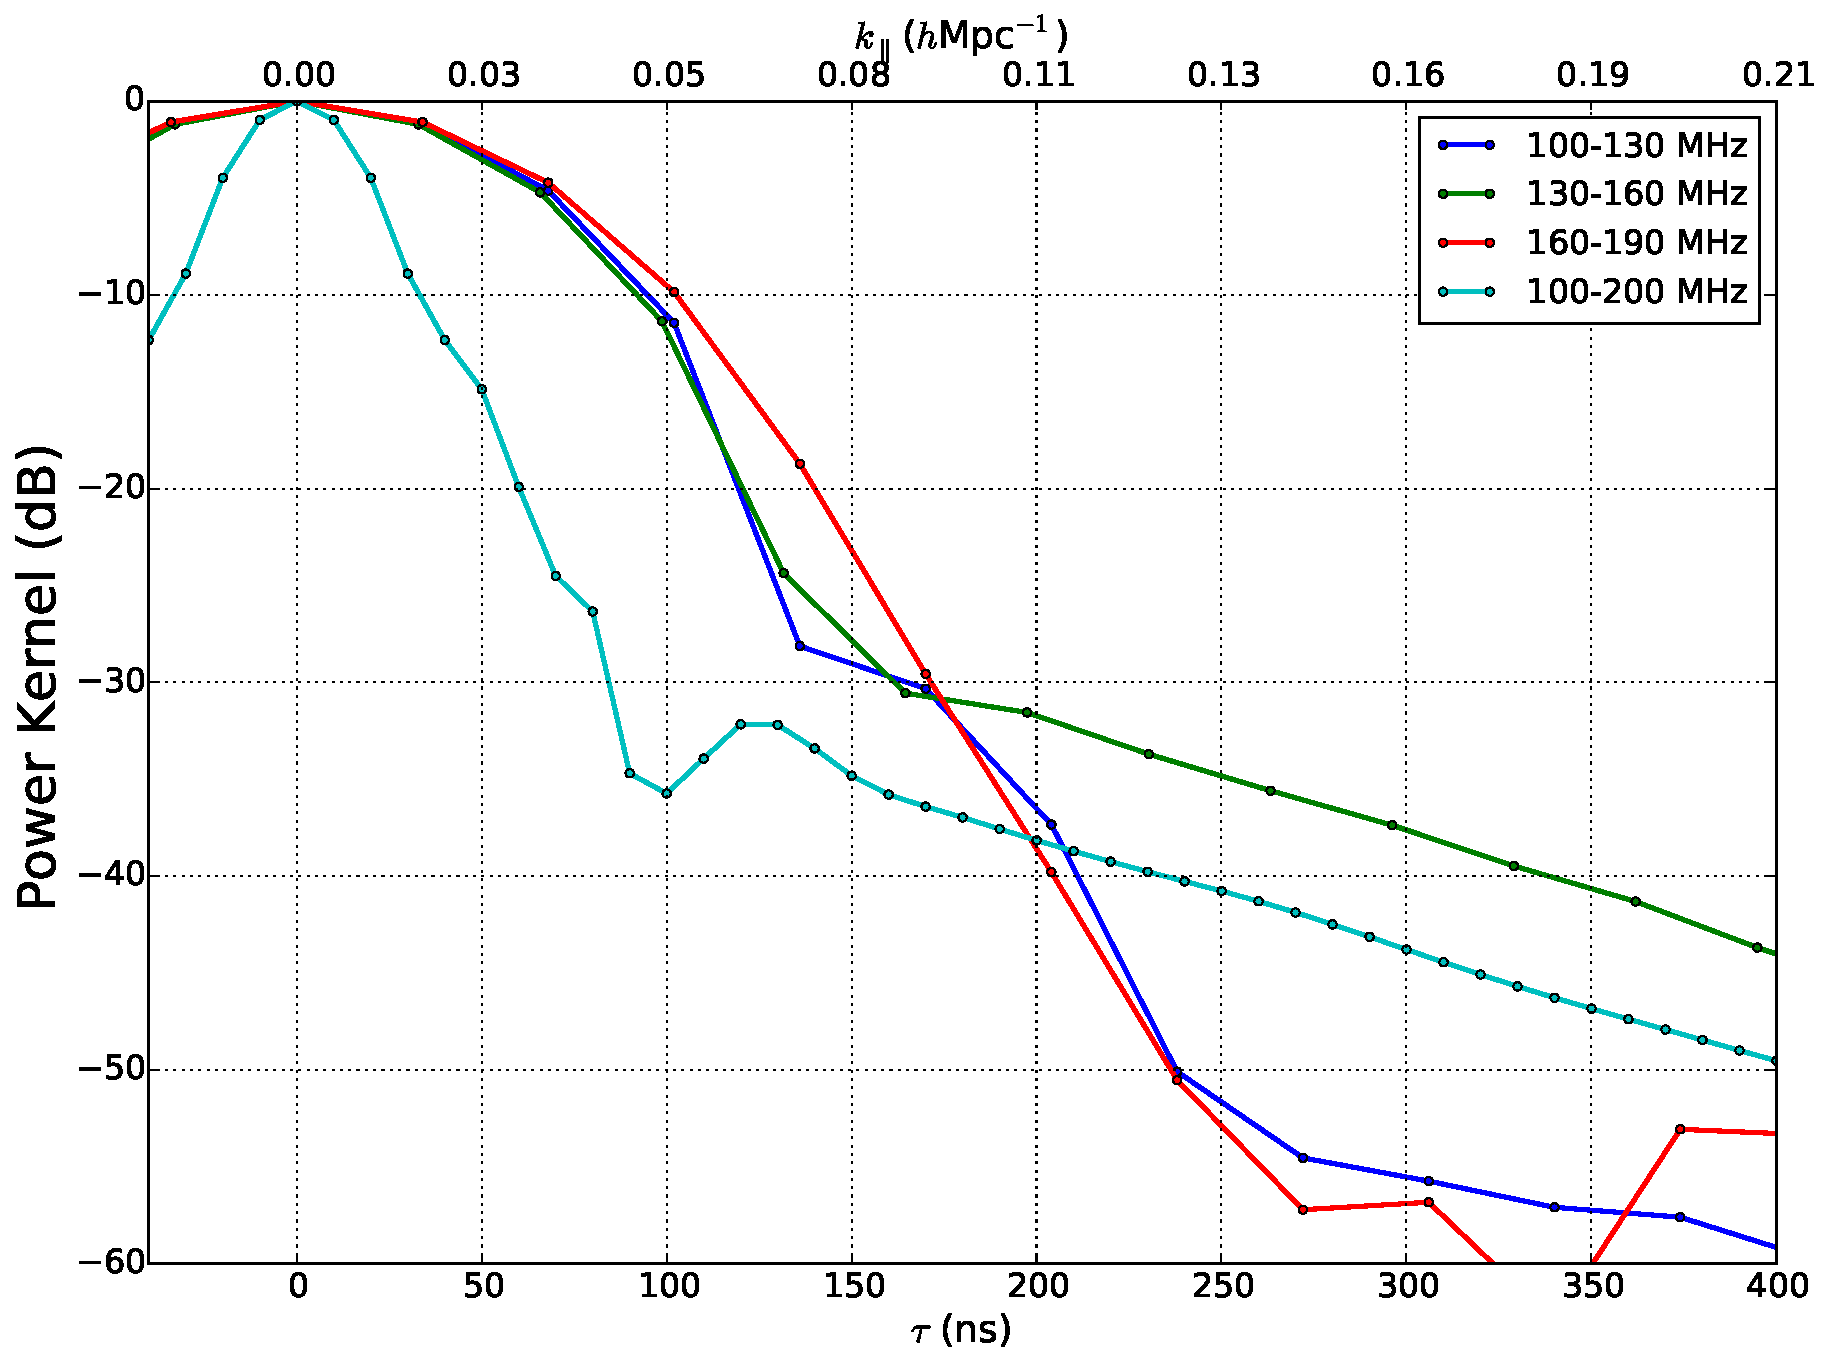
\includegraphics[width=.5\textwidth]{figures/powerKernelSubbands.pdf}
\caption{The power kernel for the three subbands discussed in in \S~\ref{ssec:Subbands} along with the kernel for the full bandwidth response function. While the long term falloff from reflections is prominent between $130-160$\,MHz, it appears at a much lower level in the other two subbands which fall below the central subband by $\sim 20$\,dB at $\sim 300$\,ns. $k_\parallel$ values for each delay are computed at $150$\,MHz. The wider central lobe below 150\,ns for the subband gains is an artifact of the delay resolution of a smaller bandwidth.}
\label{fig:KernelsSubbands}
\end{figure}

\begin{figure}
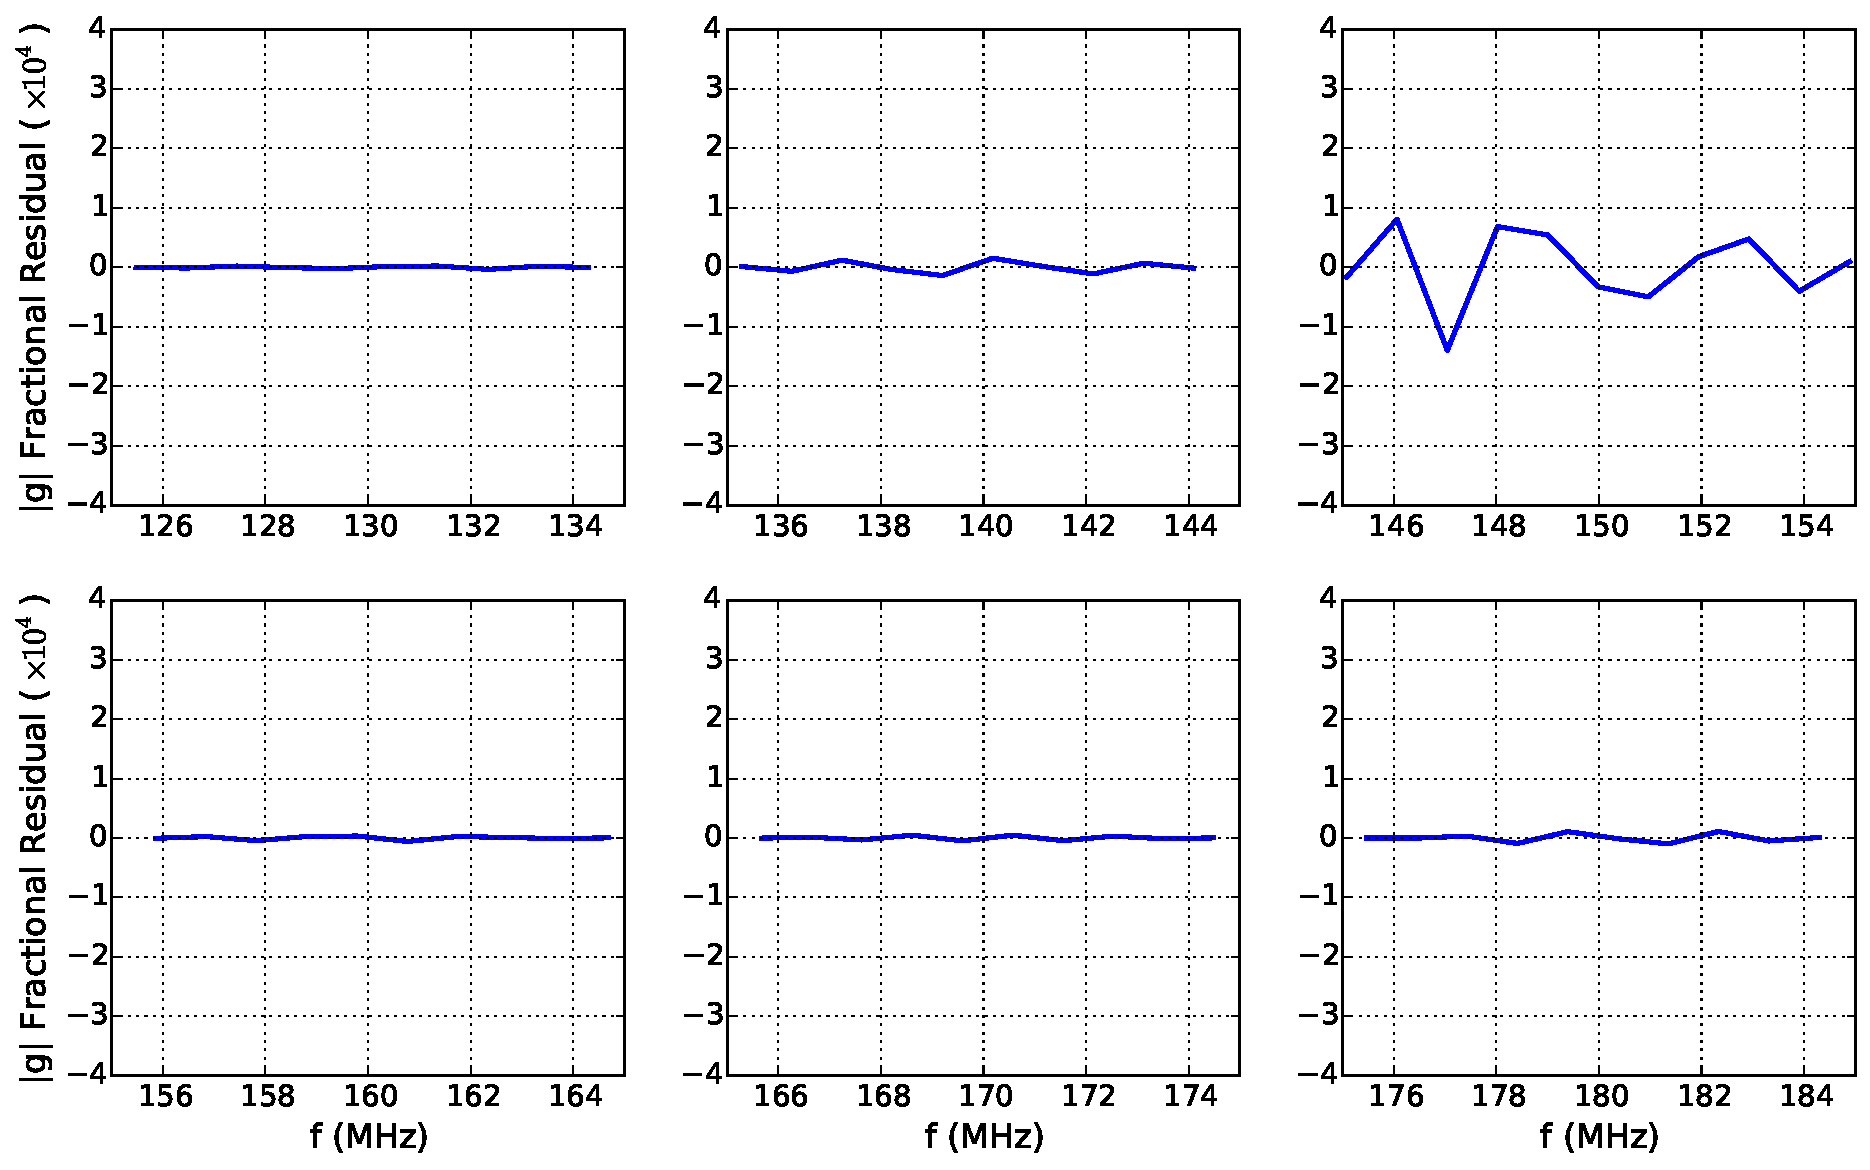
\includegraphics[width=.5\textwidth]{figures/frequency_domain_residuals.pdf}
\caption{Residuals on the absolute value of the gain over several subbands after fitting to a sixth order polynomial. Consistent with our findings in Fig.~\ref{fig:KernelsSubbands}, the fine frequency residuals in the 145-155\,MHz subband are over an order of magnitude greater than those in the other subbands.}
\label{fig:Residuals}
\end{figure}

\subsection{Verifying Our Framework with $S_{11}$ Measurements and Simulations}

We now attempt attempt to quantify the accuracy of our time-domain simulation framework by comparing simulations to measurements of the $S_{11}$ parameter of the HERA dish. Up until now, our simulations have derived the voltage response of the dish using simulations of an incoming plane wave as is the case for radio signals arriving from objects in space. It is possible to probe the gain of the dish using objects in the far field such as known radio sources \citep{Thyagarajan:2011,Pober:2012,Colgate:2015} or constellations of ORBCOMM satellites \citep{Neben:2015,Neben:2016}. However natural radio sources are too weak to probe the dish response at the $<10^{-4}$ level necessary to verify our simulations and the ORBCOMM technique can only be used to map the gain at the single frequency that the satellites transmit at, $137$\,MHz. Work is currently underway to use broad-band transmitters flown into the far field of the dish by drones \citep{Jacobs:2016} but this system is still under development. Reflectometry of the dish using a vector network analyzer is a straightforward alternative used in \citet{Patra:2016} to estimate the gains directly. Rather than comparing their estimate of the gain with our predicted gains (which is done in this paper), we instead set up a time domain simulation to compute the $S_{11}$ parameter of HERA antenna and compare it to direct $S_{11}$ measurements.
\begin{figure}
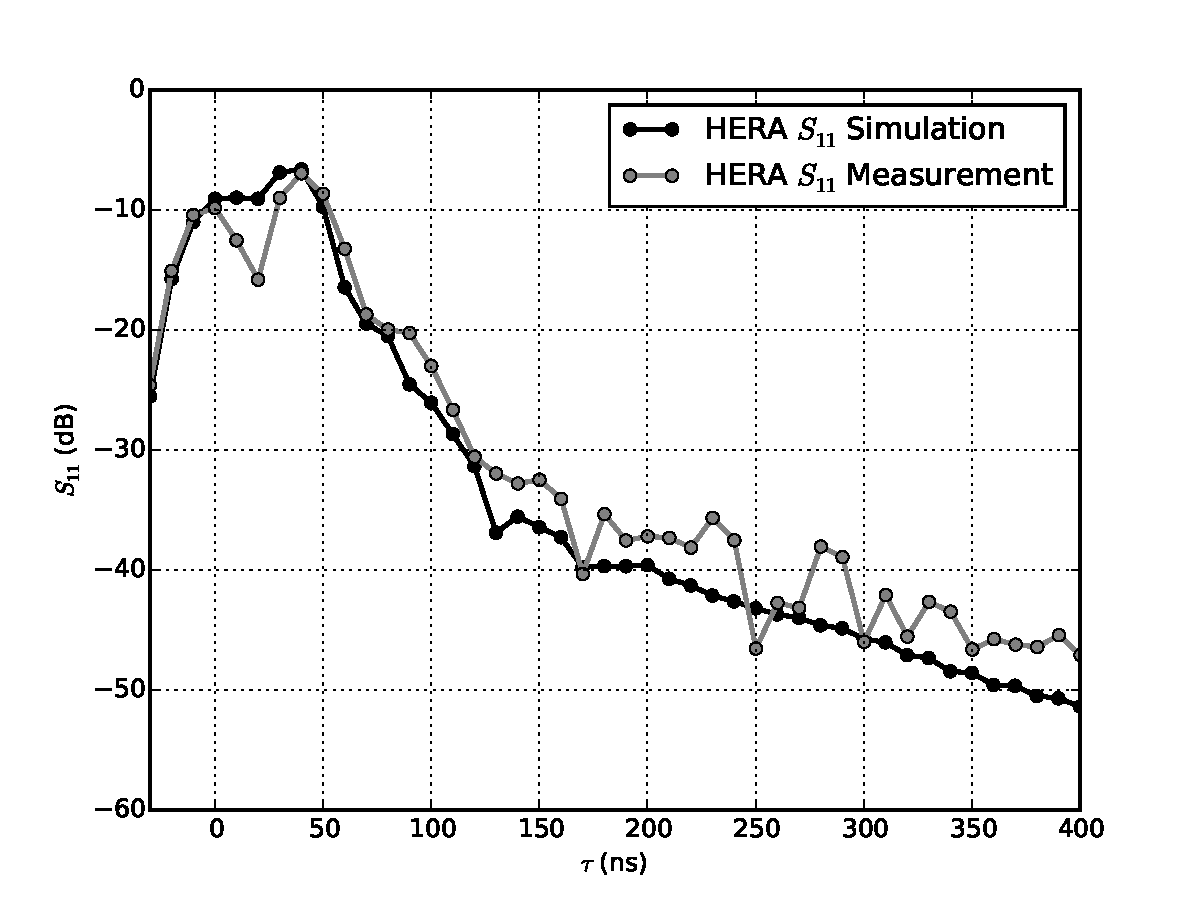
\includegraphics[width=.5\textwidth]{figures/s11_compare.pdf}
\caption{A comparison between time-domain simulations (black line) and measurements (grey line) of $S_{11}$ for the HERA dish. We also show an $S_{11}$ measurement with the cables leading from the VNA to the feed terminated by an open circuit which allows us to probe the dynamic range of the measurement. We use the standard deviation of the open measurement (grey dashed line) between $100$ and $200$\,ns as our systematic floor (grey shaded region). We find very good agreement between our $S_{11}$ measurement and the simulation, validating the predictions of our simulations.}
\label{fig:S11}
\end{figure}
For 

In our case, $S_{11}$ refers to the complex ratio between a voltage signal transmitted into the feed terminals and the voltage reflected back as a function of frequency, $ S_{11}(f) \equiv v_\text{trans}(f)/v_\text{recv}(f) $. We measure $S_{11}$ of a prototype HERA dish at the National Radio Astronomy Observatory Green Bank facility using a vector network analyzer. {\bf \color{red} Rich, fill in the details of the VNA measurement, discuss setup, VNA, measurement mode. }

Because $S_{11}$ is defined as a ratio in the frequency domain in a form identical to our voltage gains, we may run time-domain simulations similar to those described in \S~\ref{ssec:Simulations} except rather than simulating an incoming plane wave, we simulate the excitation of the feed terminals by an input voltage and record output voltage as a function of time. We obtain $S_{11}$ in the same manner that we obtained $\ftr$ using equation~\ref{eq:Inversion} with $\ftv_\text{recv}$ taking the place of $\ftv$ in the numerator inside the Fourier transform and $\ftv_\text{trans}$ taking the place of $\fts$ in the denominator. 

In Fig.~\ref{fig:S11} we show the simulated amplitude of $S_{11}$ as a function of frequency for the HERA dish and the PAPER element, observing a distinctive two peaked structure before a steep die off in delay that transitions to a shallower falloff at $\approx 150$\,ns. The first peak is due to the reflection of the input wave off of the back of the feed while the second, roughly $35$\,ns later arises from the transmitted component of the input wave reflecting off of the dish and arriving back at the feed. The ensuing long term die off arises from reflections within the feed and dish structure and for reasons that will be elaborated on in \citet{Patra:2016} corresponds very closely to our simulations of the dish gain itself (compare with Fig.~\ref{fig:SimulationResults}).  We get a sense of the dynamic range of the measurement by unhooking the SMA adapter that attaches the sleeved dipole feed to the cable from our VNA, forming an open circuit that should ideally give a reflection coefficient of $\approx 1$ at zero delay with no reflections at any other times. In this measurement, we find noise-like structure at $\approx -50$\,dB. Below $\approx 500$\,ns, we found that this structure does not integrate down upon extending the VNA integration time, leading us to conclude that it is caused by systematics, likely uncalibrated low level reflections in the VNA-feed cables. The level of this noise sets the systematic floor in our measurements which we show as a grey shaded region in Fig.~\ref{fig:S11}. We find that in the region where the $S_{11}$ measurement is above the systematics floor, there is good agreement with our simulations (within several dB) and obeying the same trends as our simulation.




\section{The Effect of the HERA dish Chromaticity on Foreground Leakage and Sensitivity}\label{sec:Sensitivity}
We are now in a position to explore the impact of the Dish's performance on the leakage of foregrounds beyond the wedge, and into the EoR window. Beyond the delay kernels considered in this paper and \citep{Patra:2016}, the extent of leakage will depend both on the angular structure of the primary beam, which is established through measurements and simulations in \citep{Neben:2016} and the brightness of the foregrounds themselves. In this section, we investigate the amplitude of foreground leakage as a function of delay given the angular primary beam model and our simulation of the delay structure of the dish. We start by extrapolating the delay structure observed in our simulations to match HERA's expected frequency resolution (\S~\ref{ssec:Extrapolation}). In \S~\ref{ssec:Leakage}, we combine this extrapolated delay response with simulations of foregrounds to determine the overall level of foreground power in HERA's visibilities. This leakage will cause large-scale LoS Fourier modes to be contaminated by foregrounds and hence inaccessible to the foreground filtering approach that HERA will employ. Since the signal-to-noise ratio is maximized at the smallest $k$ values, the loss of these modes will reduce the significance of the power spectrum detection and negatively impact the overall bottom line of the science that HERA can accomplish. We explore the impact of HERA's intrinsic beam chromaticity on science using the Fisher matrix formalism in \S~\ref{ssec:Science}. 


\subsection{Extrapolating the Bandpass and Power Kernel}\label{ssec:Extrapolation}

Our simulations of the Dish response only extend to $\approx 400$\,ns, however, we wish to understand the impact of reflections on the frequency dependent gain of an interferometer like HERA at comoving scales of $\approx 0.1-0.5$\,$h$Mpc$^{-1}$, corresponding to the delays between 180 and 900\,ns at $z=8$. To extrapolate out to higher delays, we assume that the response function is dominated by reflections between the feed and the dish. The long term falloff appears as a line on a linear-log plot (Fig.~\ref{fig:SimulationResults}), indicating that the voltage response follows an exponential which we now show is indicative of reflections. We do so by adopting the notation of \citet{Patra:2016}, letting $\Gamma_d$ represent the reflection coefficient of the Dish vertex and $\Gamma_f$ represent the reflection coefficient of the feed. An electromagnetic wave incident on the feed, at $t=0$, is accepted with amplitude $(1-\Gamma_f)$. The reflected component travels back to the dish and acquires an amplitude of $(\Gamma_f \Gamma_d)$ before returning at time, $\tau_d$ later where $(1-\Gamma_f)$ will be accepted and $\Gamma_f$ will be reflected back towards the dish. Summing the infinite series of reflections, the time dependent voltage at the feed is
\begin{equation}
\widetilde{v}_r(t) = \sum_m \left( \Gamma_f \Gamma_d \right)^m \widetilde{s}(t-m \tau_d)
\end{equation}
implying that
\begin{equation}
\widetilde{r}_r(\tau) = \sum_m \left( \Gamma_f \Gamma_d \right)^m \delta_D(\tau-m\tau_d)
\end{equation}
Since the number of reflections is $m=t/\tau_d$, than we can write the long-term delay response in discrete form as 
\begin{equation}
\widetilde{r}_n \approx (\Gamma_f \Gamma_d)^{n d\tau/\tau_d}
\end{equation}
which is an exponential in time. We thus model our discrete voltage response beyond the times sampled by our simulations as an exponential
\begin{equation}
\widetilde{r} = A X^{(\tau/30\text{ns})} 
\end{equation}
and extrapolate the time-domain voltage response of the dish by fitting for $A$ and $X$ in our simulations between 200 and 400\,ns.




\subsection{The Impact of the HERA Beam Chromaticity on Foreground Contamination}\label{ssec:Leakage}

Given the HERA dish chromaticity, what Fourier modes will still be accessible with the delay filtering technique? To answer this question, we combine our extrapolated simulations of the HERA dish's spectral structure with simulations of foregrounds. 

The foreground model is discussed in detail in \citet{Thyagarajan:2016} but we describe them briefly here for the readers convenience. It consists of two major components: diffuse synchrotron emission from our Galaxy whose structure is described by the Global Sky Model (GSM) of \citet{deOliveiraCosta:2008} and a population of point sources sourced by radio loud AGN. The point sources include those observed in both the NRAO Sky Survey (NVSS) \citep{Condon:1998} at 1.4\,GHz and the Sydney University Mologolo Sky Survey (SUMMS) \citep{Bock:1999} at 843\,MHz. Their fluxes are extrapolated to the observed $100$-$200$\,MHz band using a spectral index of $\langle \alpha \rangle=-0.83$ determined in \citet{Mauch:2003}. Visibilities are computed from the diffuse and point source models assuming an achromatic angular response for the HERA beam computed at $150$\,MHz described in \citet{Neben:2016}. We compute two sets of visibilities: one in which the spectral structure of the dish is assumed to be completely flat, and another in which the beam is multiplied by the frequency dependent gain at zenith determined by our simulations. While this model assumes incorrectly that the frequency evolution of the primary beam is identical along all lines of sight, the majority of power enters at the beams point of maximal gain and observations of autocorrelations which reflect the angular average of the frequency dependence of all lines of sight agree well with our simulations at zenith \citep{Patra:2016}. 

The foreground filtering procedure employed by PAPER and HERA involves delay transforming the visibilities and performing a 1d clean which discovers and subtract foregrounds within the horizon plus a small buffer, allowing for the suppression of foreground side-lobes in delay space. The level of foreground subtraction possible by this procedure is limited by the thermal noise level on the visibility, which in turn depends on the number of time steps and redundant baselines that are averaged before performing the cleaning step. In this work, we assume that each visibility is cleaned independently with a twenty minute cadence. Each baseline is coherent for $\approx 10$\,s per night, hence we assume that each baseline and LST is being integrated for $\approx 120$\,nights before cleaning although if we were to average over redundant baselines this number would drop enormously. The standard deviation on the real and imaginary part of a single delay transformed visibility is \citep{Morales:2004}
\begin{equation}
\sigma_V = \frac{\sqrt{2 B} k_B T_{sys}}{A_e \sqrt{\tau}},
\end{equation}
where $A_e$ is the effective area of the dish, $B$ is the bandwidth, $T_{sys}$ is the system temperature, $\tau$ is the integration time, and $k_B$ is the Boltzmann constant. For $T_{sys}$ we use the equation $T_{sys} = 100\text{K} + T_{sky}$ where $100$\,K is the temperature of the PAPER receiver and $T_{sky} = 60 (\lambda/1\,\text{meter} )^{2.55}$ is the sky temperature \citep{Fixsen:2011}. For $A_e$ we use the value of $98$\,m$^2$ determined in \citet{Neben:2016}. We assume that cleaning is performed down to five times the thermal noise level. In Fig~\ref{fig:Cleaning} we compare the delay transform of visibilities before and after cleaning at the LST of 4 hours. While cleaning is able to remove structure within the horizon, it does not reduce any of the power leaked outside of the horizon by the chromaticity of the dish. 

To form estimates of the 21\,cm power spectrum, we split each visibility into Blackman-Harris windowed sub-bands centered at redshift intervals of $\Delta z = 0.5$ and each with a power equivalent bandwidth of $10$\,MHz\footnote{The end to end width of each Fourier transformed interval is 20\,MHz, however the effective width of this interval is only $\approx 0.5$ the full width since the Blackman-Harris window supresses the edge channels.}, corresponding to the redshift interval over which the statistics of the brightness temperature fluctuations are expected to be stationary. The flat sky approximation allows us to Fourier transform each interval in frequency, square, and multiply by a set of prefactors to obtain a power spectrum estimate \citep{Parsons:2014},
\begin{equation}\label{eq:PS}
\widehat{P}({\bf k}) = \left( \frac{2 k_B}{\lambda^2} \right)^2 \frac{X^2 Y}{B_{pp} \Omega_{pp}} | \widetilde{V}({\bf u}) |^2.
\end{equation}
Here, $\lambda$ is the central wavelength of the observation, $k_B$ is the Boltzmann constant, $B_{pp}$ is the integral of the square of the bandpass, and $\Omega_{pp}$ is the integral of the primary beam squared over solid angle. $X$ and $Y$ are linear factors converting between native interometry and cosmological coordinates, defined through the relation $2 \pi {\bf u}=2 \pi (u,v,\eta) = (X k_x, X k_y, Y k_z)$. 

A drift scan instrument, HERA will be capable of observing the sky at any LST within the strip declination that passes through its primary beam. To form a final power spectrum estimate, it is expected to perform an average over the power spectrum estimates for each LST. It is well documented that foreground power varies significantly over LST \citep{Thyagarajan:2015a}, hence such an estimate will either filter or weight LSTS in a way that minimizes the impact of the most contaminated observations. For our analysis, we focus on a single LST of 4 hours which points out of the galactic plane and represents a relatively clean pointing similar to those we expect for HERA to concentrate its observing time on.  




\begin{figure}
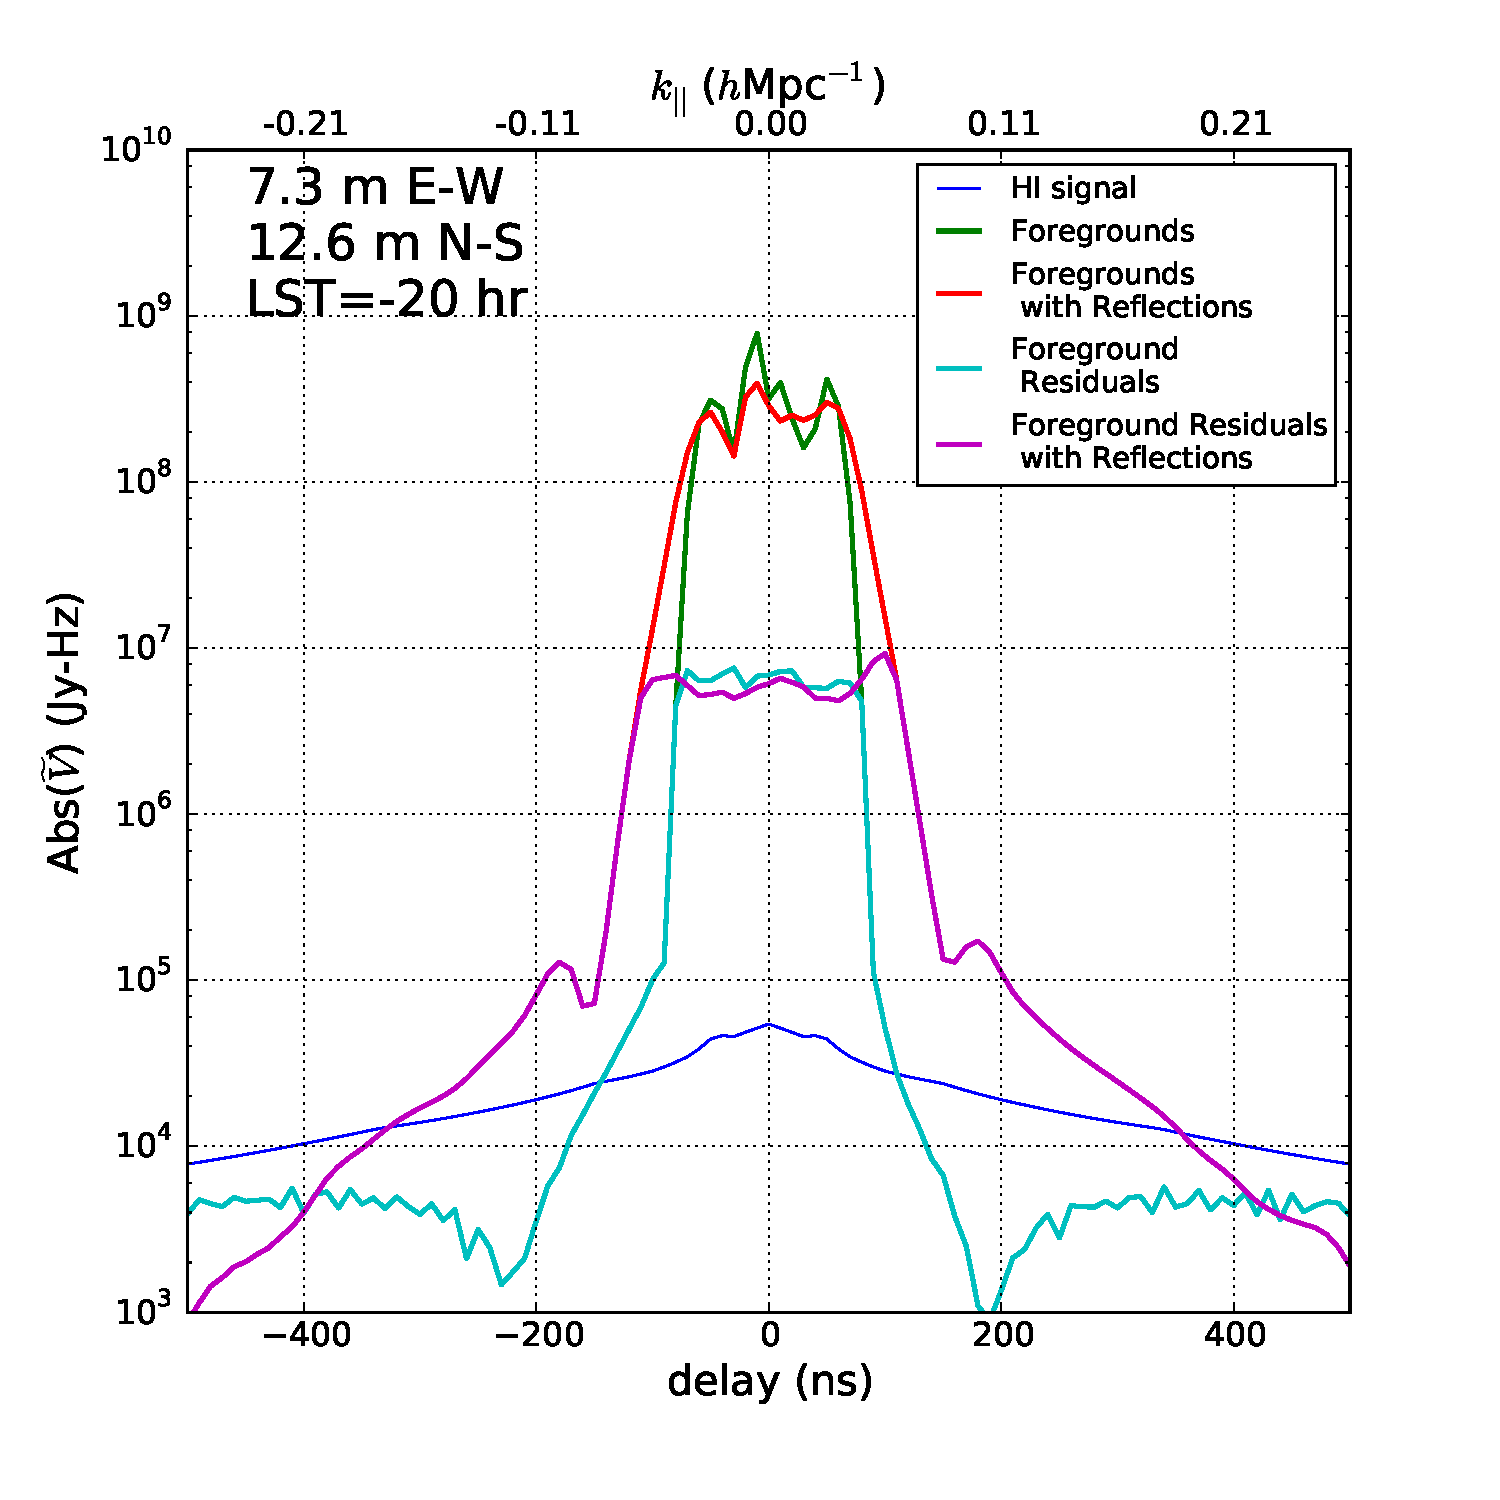
\includegraphics[width=.5\textwidth]{figures/cleaning_noise_Nithya.pdf}
\caption{The absolute magnitude of a delay transformed 14-meter baseline (blue line) compared to the same visibility (green line) contaminated by reflections at the level observed in the HERA dish design. We see that the extended delay kernel smooths out structure, originating from foregrounds, within the horizon. For HERA, we expect to use the delay-clean to remove foregrounds. However, the depth of cleaning is limited by the noise level on a single baseline (black line). We show the foreground residuals with arising from a clean down to the $5\,\sigma$ noise level after 2 minutes of integration, seeing that cleaning at this cadence achieves $\approx$ two orders of magnitude of foreground reduction. The reflections in the dish lead to extensive winged structures that bleed into the EoR window and are well below the thermal noise level. All data in this plot are obtained from a $100$\,MHz bandwidth centered at $150$\,MHz. Vertical dashed lines indicate the horizon delays of the baseline.}
\label{fig:Cleaning}
\end{figure}


Computing the power spectra, we inspect the amplitude of foregrounds given the chromaticity and angular pattern of the HERA dish for baselines of two different lengths in Fig.~\ref{fig:BothBaselines}. In both baselines, we find that the residuals after cleaning tend to be at similar levels except at the subband centered at $z=8.5$ (150\,MHz), in which foreground residuals remain above the signal level out to $k_\parallel=0.23$\,$h$Mpc$^{-1}$. Several other baselines especially those oriented entirely in the E-W direction, which we do not show, contain up to two orders of magnitude greater galactic  contamination as is noted in \citet{Thyagarajan:2015b}. In an analysis, these baselines would be down-weighted or discarded so that they do not bias our final estimate. 

The level of the foregrounds in Fig.~\ref{fig:BothBaselines} is conservative since no attempt has been made to apply inverse covariance weighting techniques \citep{Tegmark:1997a,Liu:2011,Dillon:2013,Parsons:2014,Liu:2014a,Liu:2014b,Dillon:2015a,Dillon:2015b,Trott:2016} or fringe rate filtering \citep{Parsons:2015}. In order to avoid biases in a maximum likelihood analysis that determines astrophysical and cosmological parameters from our power spectra, the foregrounds should ideally be below the anticipated level of thermal noise which is shown in \citet{Pober:2014} to be on the order of a few percent the anticipated level of the cosmological signal for the full HERA deployment. Hence, as long as we can suppress our foregrounds below $\approx 1$\% the level of the signal, they should not interfere significantly with a maximum likelihood analysis. Thus, the residuals in Fig.~\ref{fig:BothBaselines} serve as a specification for any inverse covariance weighting pipeline which will need to suppress foregrounds by between a factor of $\sim 1-10$ to bring the worst contaminated regions below the level of the signal. Applications of inverse covariance filters in recent PAPER observations have yielded improvements at and above this level {\bf \color{red} citation?}, hence our simulations show that even with the presence of beam chromaticity, HERA will be able to isolate foregrounds below the level of thermal noise in most of the EoR window. 

\begin{figure*}
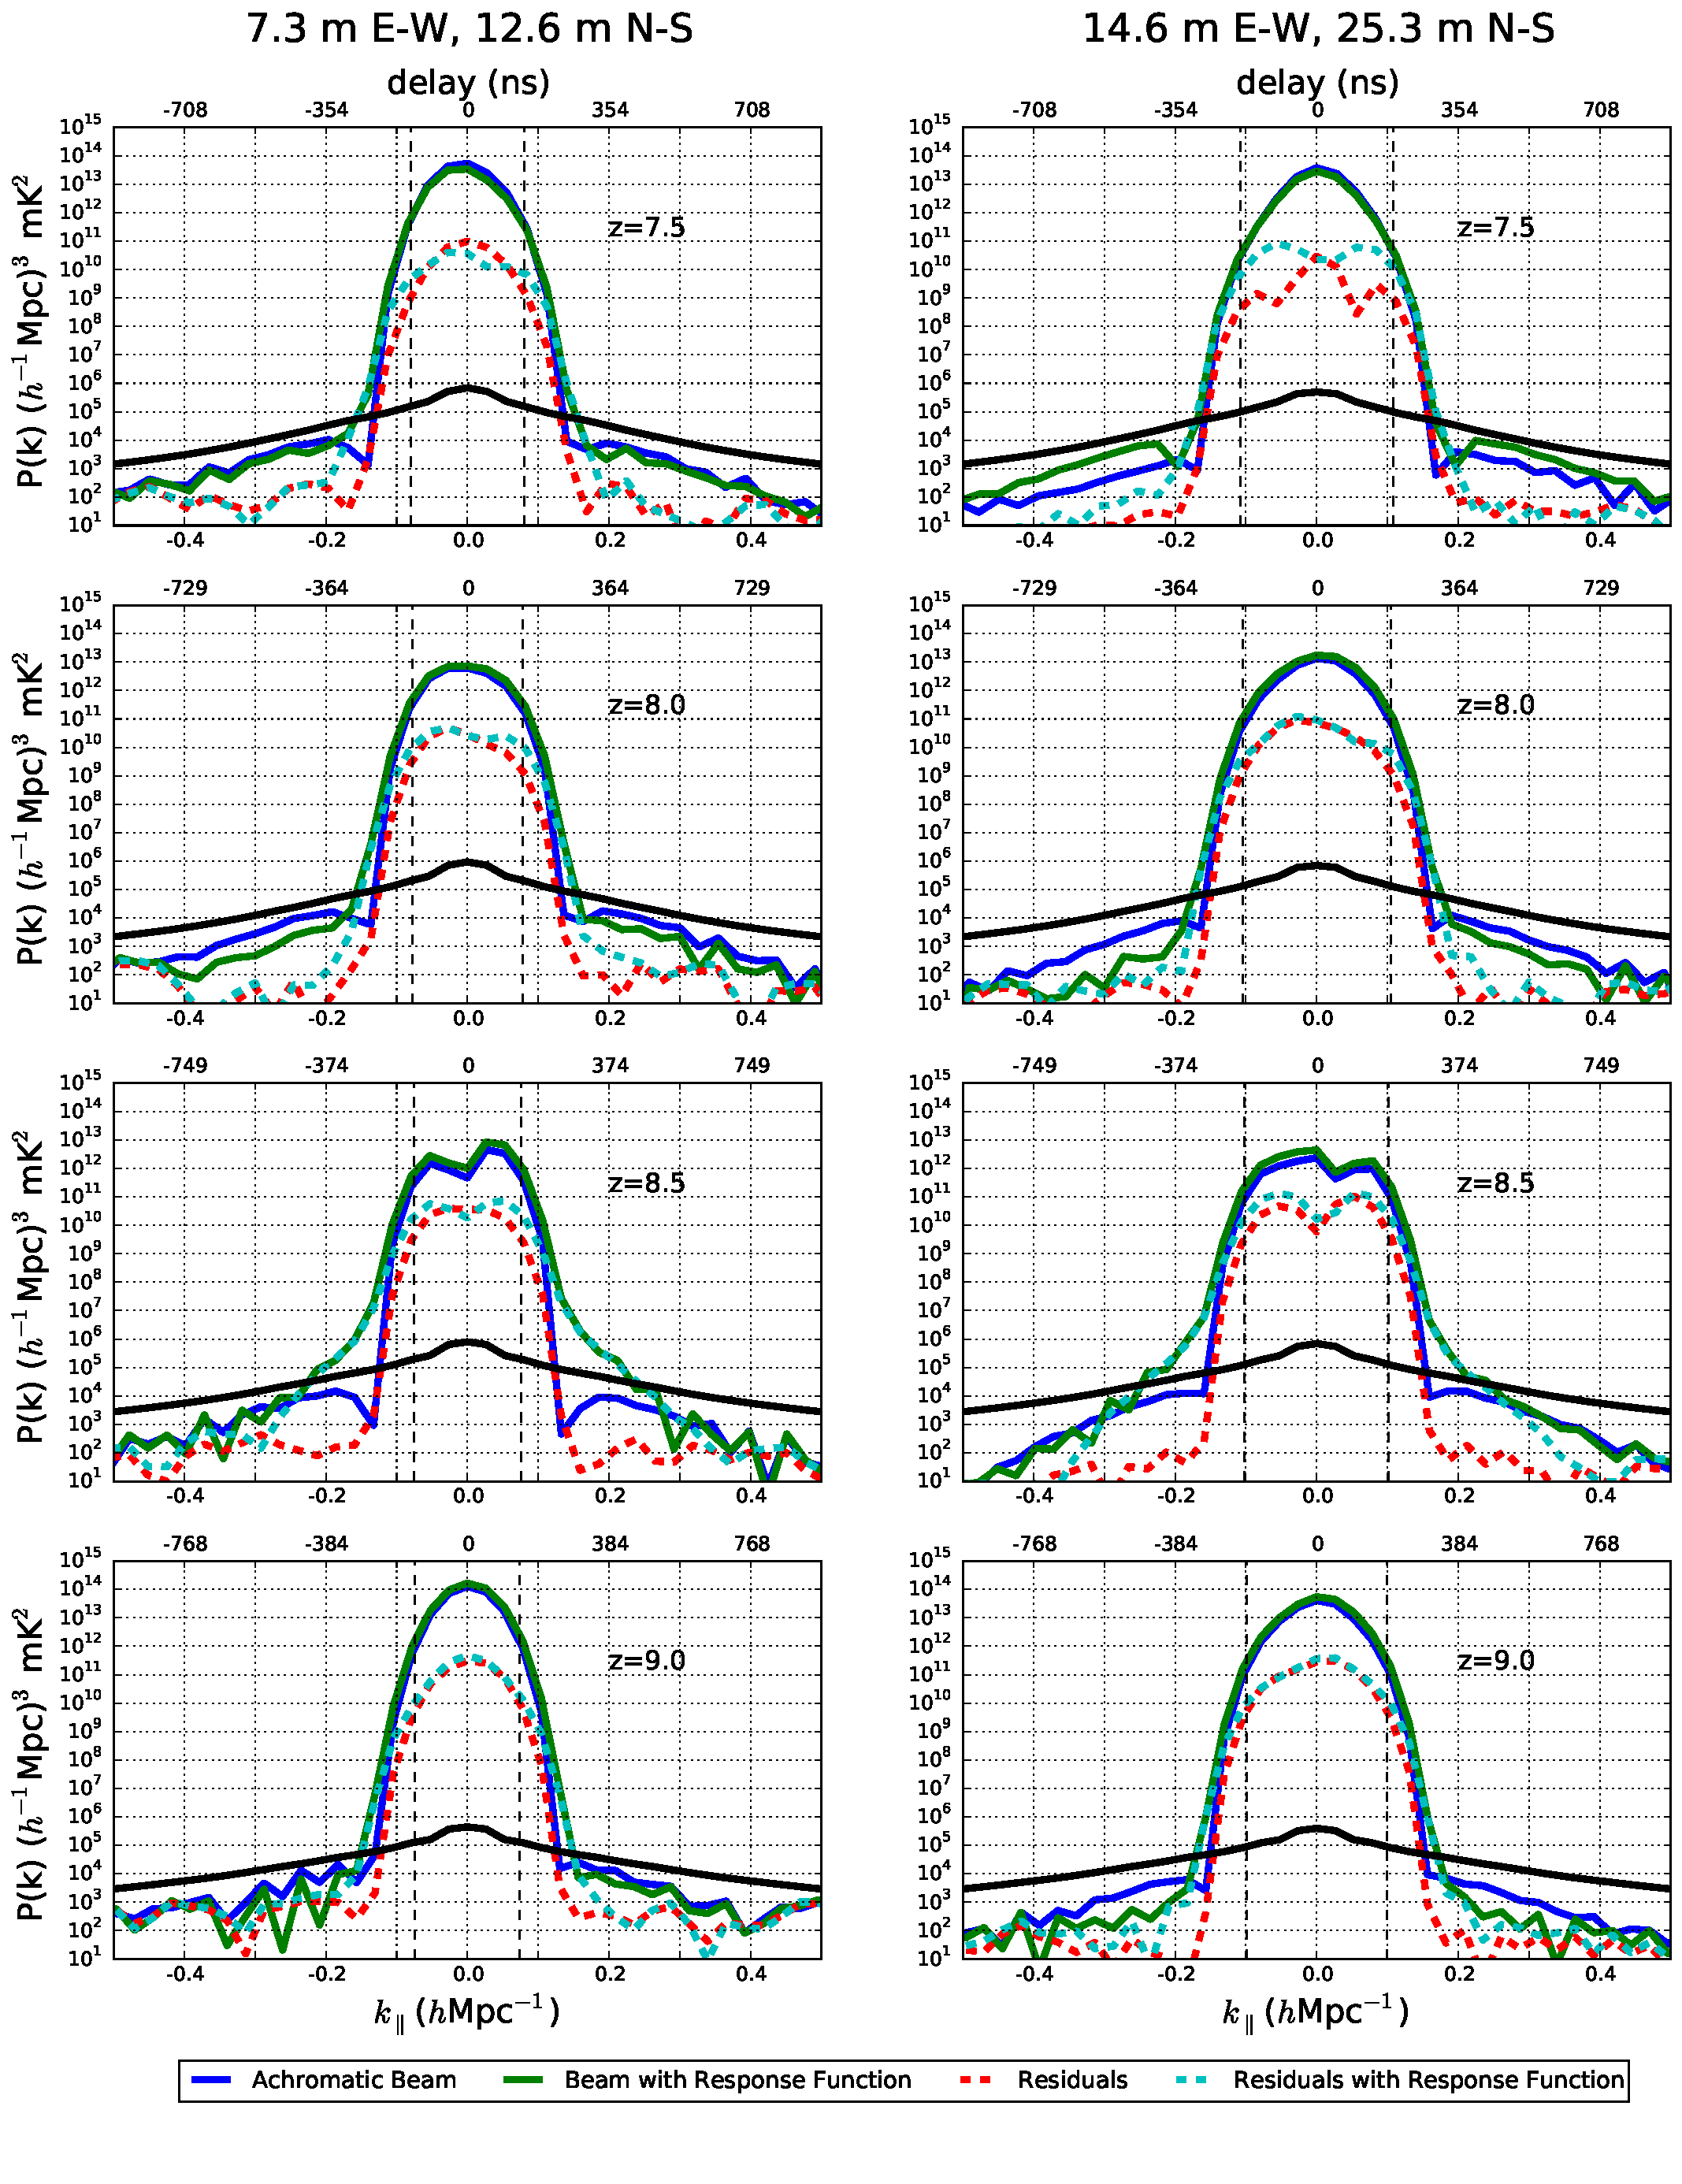
\includegraphics[width=\textwidth]{figures/ps_compare_nithya_bothBaselines.pdf}
\vspace{-24pt}
\caption{The delay transform power spectrum for different baselines over several redshifts with (green solid line) and without (blue solid line) the presence of the simulated chromaticity in the HERA dish. Each estimate is computed using the square of a Blackman-Harris windowed  delay transform (equation~\ref{eq:PS})) over an equivalent power bandwidth of $10$\,MHz. We also show the power spectra of foreground residuals after cleaning the entire $100$\,MHz band with (dashed cyan line) and without (red dashed line) the beam spectral structure. For all subbands except $z=8.5$, we find that the reflections in the HERA dish have a negligible effect on the $k_\parallel$ where the foregrounds drop below the signal level. This is the same subband where enhanced spectral structure due to reflections are observed in our simulations (Figs.~\ref{fig:KernelsSubbands} and \ref{fig:Residuals}).}
\label{fig:BothBaselines}
\end{figure*}






\subsection{The Implications of Dish Reflections on EoR Science}\label{ssec:Science}
A primary near-term goal of 21\,cm EoR observations is to obtain information about the nature of the sources that drove reionization. Since the amplitude of the 21\,cm signal is maximal at smaller $k$ values, a loss of large scale signal due to foreground contamination eliminates the the modes that HERA would otherwise have the greatest signal to noise detections of, reducing its overall sensitivity. In this section, we use the Fisher Matrix formalism to estimate the impact of foreground leakage on HERA's sensitivity along with its ability to determine the astrophysics of reionization. The Fisher Matrix allows us to forecast the covariances and errors on reionization parameters given errors on power spectrum observations due to the uncertainties caused by cosmic variance and thermal noise which is in turn determined by the $uv$ coverage and observing time of the interferometer. The covariance between the parameters of some model ${\bf \theta}$ is given by the inverse of the Fisher matrix, ${\bf F}$ which for Gaussian and independently determined power spectrum bins may be written approximately as \citep{Pober:2014},
\begin{equation}\label{eq:Fisher}
F_{ij} \approx \sum_{k,z} \frac{1}{\sigma^2(k,z)} \frac{\partial \Delta^2(k,z)}{\partial \theta_i} \frac{\partial \Delta^2(k,z)}{\partial \theta_j},
\end{equation}
where $\Delta^2(k,z)$ is the power spectrum amplitude for some $k-z$ bin and $\sigma^2(k,z)$ is the variance of the power spectrum estimate in that bin due to thermal noise and cosmic variance \citep{Beardsley:2013}. We write this equation as approximate since it ignores terms arising from the dependence of $\sigma^2(k,z)$ on model parameters due to cosmic variance but only contribute at the $\approx 1$\% level \citep{EwallWice:2015b}. 

To simulate $\Delta^2$, we use the publicly available {\tt 21cmFAST}\footnote{\url{http://homepage.sns.it/mesinger/DexM___21cmFAST.html}} code \citep{Mesinger:2011} which generates realizations of the 21\,cm brightness temperature field using the excursion set formalism of \citet{Furlanetto:2004}. We employ a popular three parameter model of reionization \citep{Mesinger:2012} with the following variables 
\begin{itemize}
\item ${\bf \zeta}$: The ``ionization efficiency" is defined in the \citet{Furlanetto:2004} excursion formalism to be the inverse of the mass collapse fraction necessary to ionize a region and is computed from a number of other physical parameters including the fraction of collapsed baryons that form stars and the UV photon escape fraction. Because $\zeta$ acts as an efficiency parameter, its primary affect is to change the timing of reionization. We choose a fiducial value of $\zeta=20$, though its possible values range anywhere between $5$ and $50$. 
\item ${\bf R_\text{mfp}}$: The presence of Lyman limit systems and other potential absorbers within HII regions causes UV photons to have a mean free path denoted by $R_\text{mfp}$. In the {\tt 21cmFAST} framework, HII regions cease to grow after reaching the radius of $R_\text{mfp}$, primarily impacting the morphology of the signal. We choose a fiducial value of $R_\text{mfp}=15$\,Mpc which is in line with recent simulations accounting for the subgrid physics of absorption \citep{Sobacchi:2014}. 
\item ${\bf T_\text{vir}^\text{min}}$: The minimal mass of dark matter halos that hosted ionizing sources. While in principle, halos with virial temperatures as small as $10^2$\,K are thought to be able to form stars \citep{Haiman:1996a,Tegmark:1997c}, thermal and mechanical feedback have been seen to raise this limit to as high as $10^5$\,K \citep{Springel:2003,Mesinger:2008,Okamoto:2008}. We choose a fiducial value of $T_\text{vir}^\text{min} = 1.5\times 10^4$\,K which is set by the atomic line cooling threshold. 
\end{itemize}
In order to account for the degeneracies in the power spectrum between heating from X-rays and reionization from UV photons, we also marginalize over three additional parameters that describe the impact of heating from early X-ray luminous sources as explored in \citep{EwallWice:2015b}. These are the X-ray heating efficiency $f_X$, the maximal energy of X-ray photons that are self absorbed by the ISM of early galaxies, $\nu_\text{min}$, and the spectral slope, $\alpha$ which are taken to have fiducial values of $1$, $0.3$\,keV, and $-1.2$ respectively. We choose to parameterize our model in terms of the fractional differences of each parameter from their fiducial values so that, for example, $\theta_\zeta = (\zeta - \zeta_\text{fid})/\zeta_\text{fid}$ and compute the derivatives in equation~\ref{eq:Fisher} by performing a linear fit to realizations of the 21\,cm power spectrum calculated by {\tt 21cmFAST} at $\theta_i= \pm 10^{-2}, \pm 5\times 10^{-2}, \pm 10^{-1}$,and $ \pm 2 \times 10^{-2}$. 

What about $\sigma^2(k,z)$? For each measurement in the $uv$ plane, the standard deviation of a power spectrum measurement is given by the direct sum of sample variance and thermal noise \citep{McQuinn:2006} which in turn depends on the primary beam of the instrument and the time spent sampling each $uv$ cell. For our analysis, we assume that the $uv$ plane is sampled by circular apertures with effective areas of $98$\,m$^2$ and that $\tau({\bf k})$ is determined by a drift scan in which non instantaneously redundant baselines are combined within each $uv$ cell. We compute the sensitivity for the proposed 331-element hexagonally packed deployment of HERA (HERA-331). 


\begin{figure}
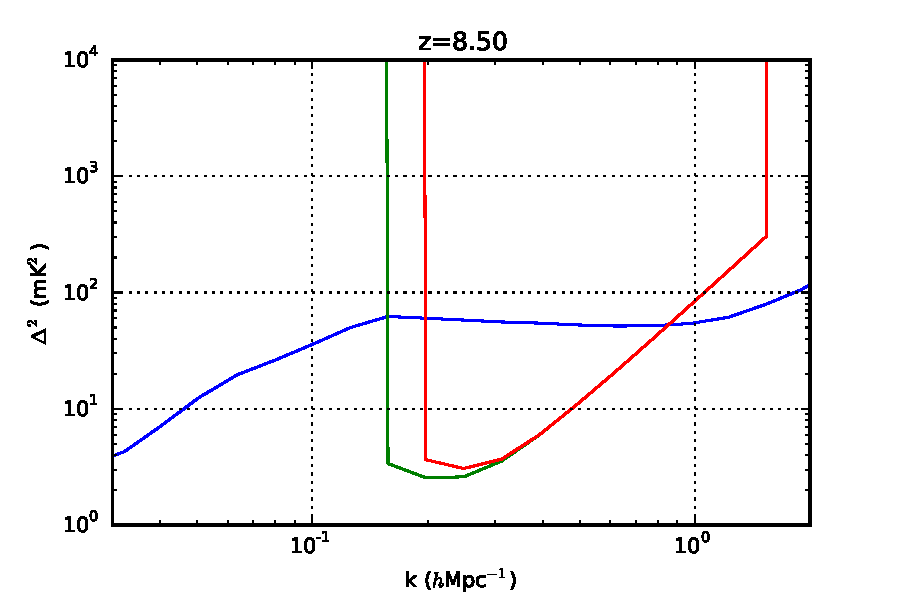
\includegraphics[width=.5\textwidth]{figures/sensitivity_comparison_v2.pdf}
\caption{A comparison between the sensitivity achieved by HERA-331 at redshift $8.5$ with and without the presence of beam chromaticity due to the reflections studied in this work. We saw in Fig.~\ref{fig:BothBaselines} that with reflections, foregrounds exceed the signal level out to $k=0.23$\,$h$Mpc$^{-1}$ at $z=8.5$ which we assume are unusable, forcing us to ignore modes out to $350$\,ns beyond the horizon, leading to the sensitivity projected in the red curve. The absence of these reflections allows us to work within $250$\,ns of the horizon (green curve), leading to an increase in sensitivity by a factor of $\approx 1.5$. }
\label{fig:Sensitivity}
\end{figure}



\begin{figure*}
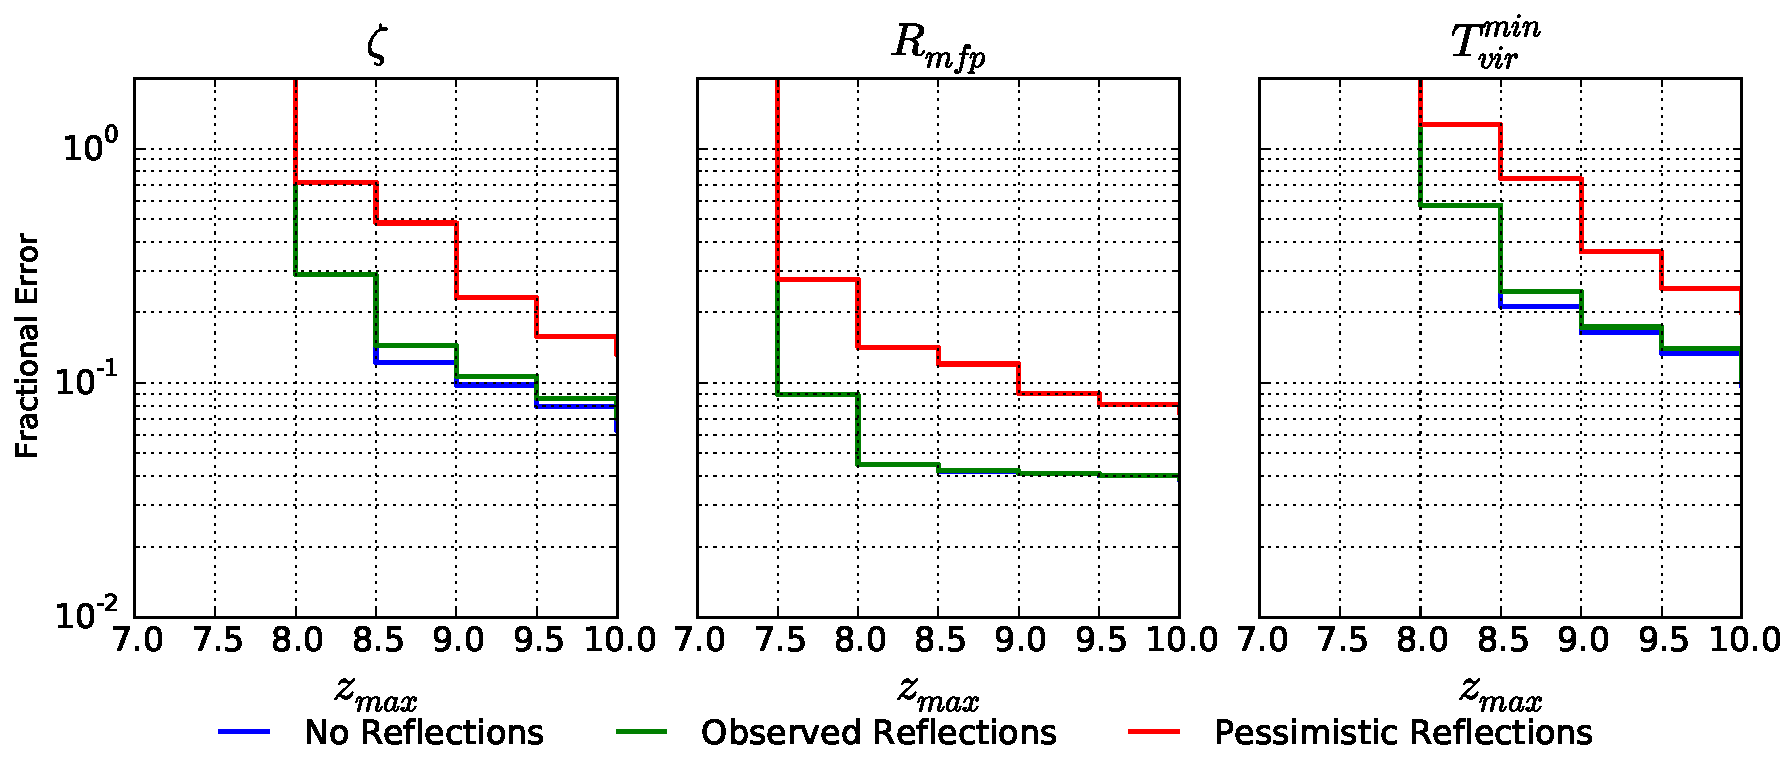
\includegraphics[width=\textwidth]{figures/sigmaVsZ_reionization_v2.pdf}
\caption{Fractional Errors on reionization and heating parameters as a function of maximal observed redshift out to the low end of HERA-331's initial observing band at $z=12$. The presence of strong reflections contained within a small subband at $z=8.5$ has a minimal impact on our overall constraints on reionization parameters. If these reflections are not localized they can lead to a factor of two loss in sensitivity to some parameters such as $T_\text{vir}^\text{min}$.}
\label{fig:Errors}
\end{figure*}

\begin{figure}[h!]
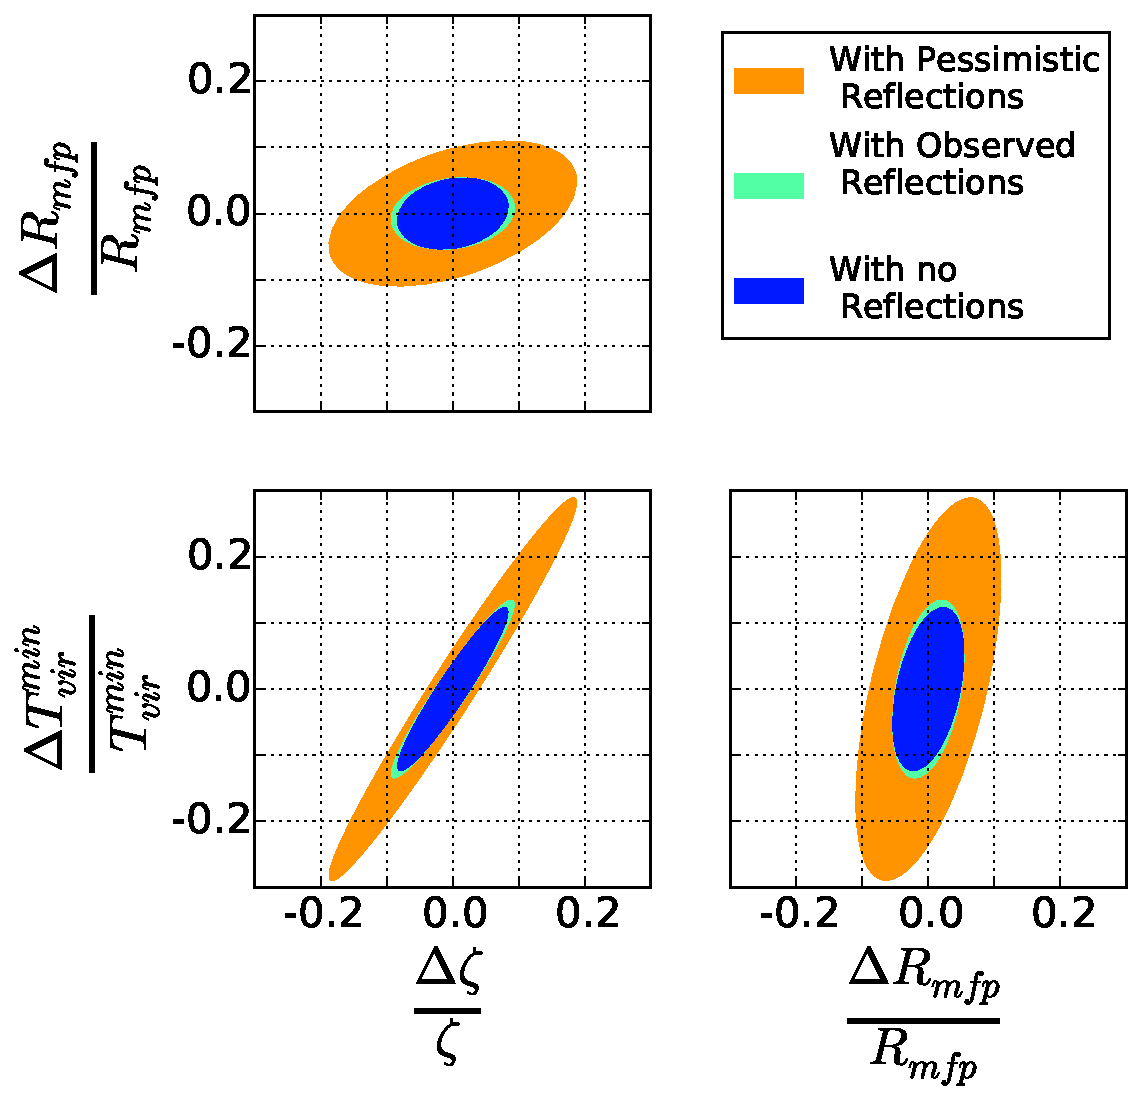
\includegraphics[width=.5\textwidth]{figures/reionization_triangle_compare_v2.pdf}
\caption{95\% confidence regions for reionization parameters assuming $1000$ hours of observation on HERA-331 between the redshifts between 7.5 and 12. The presence of the reflections leads to an increase in the major axes of these confidence regions by a factor of one to two.}
\label{fig:Confidence}
\end{figure}


We have seen in Fig.~\ref{fig:BothBaselines} that the simulated chromaticity of the dish leaks foregrounds beyond the horizon to varying degrees depending on the subband with the worst leakage occuring at $z=8.5$ centered at 150\,MHz in which foregrounds exceed the signal out to $\sim 380$\,ns which for a $14.6$\,m baseline is $\approx 330$\,ns beyond the horizon. At all other redshifts, the leakage due to beam chromaticity only extends to $\approx 250$\,ns beyond the horizon. To determine the impact of our observed beam chromaticity on HERA's ability to constrain the astrophysics of reionization, we consider three different scenarios for beam chromaticity that capture a range of possibilities informed by our simulations. 


\begin{itemize}
\item {\bf Optimistic: The observed reflections are an artifact of the simulation.} It is possible that the long term reflections observed in the center of our gain are artifacts of our modeling such as dissipative effects due to unmodeled non-idealities in the geometry of the disk will allow reflected radio waves to be better absorbed or escape into space. In our most optimistic scenario, we assume their absence in which case the foregrounds pass below the level of the signal at $250$\,ns beyond the horizon at all redshifts between $z=7$ and $12$, consistent with what is observed in the bands where the dish chromaticity is less severe or when it is not present at all. We do not consider the possibility that optimal inverse covariance weighting of the foregrounds  may actually decrease the minimal delays accessible to below the $250$\,ns above the horizon observed in our simulations. Hence, this scenario is actually somewhat conservative and certainly more pessimistic than the ones considered in \citet{Pober:2014,Liu:2015a,Liu:2015b,EwallWice:2015b}. 
 
\item {\bf Moderate: The Simulations accurately capture the chromaticity of the dish.} In this case, we assume that the reflections cause foregrounds to pass below the level of the signal at $250$\,ns beyond the horizon except at redshift $8.5$ where they pass below the foregrounds at $350$\,ns beyond the horizon. 


\item {\bf Pessimistic: The reflections are present in all sub-bands.} In this scenario, we assume that the spectral structure observed in the neighborhood of $150$\,MHz is present throughout the entire $100$-$200$\,MHz frequency range covered by HERA. While more pessimistic than anything we actually observe in our simulations, this scenario serves as a reasonable upper bound on the reflections we expect given our simulations.
 
\end{itemize}
In Fig.~\ref{fig:Sensitivity}, we compare the level of $1\sigma$ thermal noise for our optimistic and moderate scenarios at $z=8.5$ to the amplitude of the 21\,cm signal. While the level of thermal noise monotonically increases with $k$, there is a small upturn at the smallest $k$ values due to an increase in sample variance caused by the knee like maximum in the 21\,cm power spectrum at $k \approx 0.1$\,$h$Mpc$^{-1}$ and the shrinking number of measurements within each 1d $k$-bin. Despite this upturn, the smallest $k$ modes are still the highest signal to noise measurements that HERA is expected to obtain, leading to a reduction in the maximal signal to noise ratio of $\approx 1.5$ and a reduction in the number of modes that the instrument is able to measure. 

Folding our calculations of thermal noise and the derivatives of $\Delta^2$ into equation~\ref{eq:Fisher} and inverting, we obtain the covariance matrix for model parameters. We show the 95\% confidence ellipses for the reionization parameters in Fig.~\ref{fig:Confidence}. The presence of reflections within a limited sub-band about $z=8.5$ leads to an almost neglible increase in the extent of our confidence intervals while the presence of the reflections across the entire band causes the length and width of our confidence ellipses to increase by a factor of $\approx 2$. The diagonal elements of our covariance gives us error bars on each parameter which we plot in Fig.~\ref{fig:Errors}. We see that similar to our confidence regions, the error bars on reionization parameters for our optimistic and moderate scenarios are nearly indestinguishable. In our worst case where reflections of a similar level as observed in the middle of our band are present everywhere, we see an increase in our error bars by a factor of $\approx 2$. 

The error bars on reionization parameters, even for our most optismtic model, are a factor of a few larger than the ``moderate" errors predicted in previous works using likelihood analyses such as \citet{Pober:2014}, \citet{Greig:2015,Greig:2015b,Greig:2015c}  \citet{EwallWice:2015b}, \citet{Liu:2015a,Liu:2015b}. There are several reasons for this. Firstly, in our most optimistic scenario, we assumed that foregrounds cause the signal to be inaccessible below $250$\,ns beyond the edge of the wedge while in all previous works, a comoving $k$ of $k_\text{min}=0.1$\,$h$Mpc$^{-1}$, rather than a delay was used. This delay corresponds to a larger comoving wave number of $k\approx0.15$\,$h$Mpc$^{-1}$ at $z=8.5$. Secondly, previous studies assumed a fully illuminated HERA aperture, which for a $14$\,m dish predicts and effective area of $\approx155$\,m$^2$. Electromagnetic simulations and ORBCOMM mapping of the angular beam pattern of the HERA dish show that the effective area of the antenna element is actually $\approx 98$\,m$^2$ at $137$\,MHz which leads to an increase in the overall thermal noise levels by a factor of $\approx 1.5$ \citep{Neben:2016}. 

Although conservative, our predictions bode well for the HERA design, indicating that even with the additional systematics introduced by the Dish geometry, the array will still obtain a $\gtrsim 10 \sigma$ detection of the power spectrum and be capable of establishing precision constraints on the properties of reionization galaxies. 

\section{Conclusions}\label{sec:Conclusion}
In this paper, we have formally described the impact of instrumental chromaticity on foreground contamination of the 21\,cm signal. We have also used simulations of electromagnetic waves incident from zenith on the primary antenna element on HERA to determine the extent to which reflections and other frequency dependent structure in the dish that might leak foregrounds into the EoR window. The results of our simulations of the dish's voltage response are broadly consistent with reflectometry measurements \citep{Patra:2016} and can be summarized in the following points. 
\begin{itemize}
\item The 14-m dish and inverted dipole feed configuration introduces reflections and, as a result, spectral structure, that is in excess of that observed in the antenna design for HERA's predecessor, PAPER. The dish design is intended to greatly increase array collecting area over PAPER without significantly raising the number of correlated elements while narrowing the angular field of view and suppressing the overall amplitude of foregrounds. We find that in achieving these ends, some degree of spectral smoothness has been sacrificed. Because foreground filtering in delay space cannot distinguish between signal and foregrounds, any regions of $k$-space contaminated by these reflections are effectively unusable in a 21\,cm measurement unless they can be modeled to high fidelity and removed. 

\item Fortunately, these reflections appear to be contained within the central $10$\,MHz of the HERA band, indicating a resonance that, in principle can be identified in the dish design and mitigated. It is also possible that the  non-ideal properties of an actual antenna will allow these reflections to escape the dish after a short time or be dissipated, rather than reflecting continually to long delays. Because estimates of the power spectrum are obtained from sub-intervals of $\approx10$\,MHz, the reflections that we have simulated will only impact a single $\Delta z=0.5$ redshift interval.

\item Simulating the impact of these reflections on foreground leakage using the foreground model of \citet{Thyagarajan:2016}, we find that the beam chromaticity extends foregrounds above the level of the cosmological signal to $\approx 350$\,ns beyond the horizon while without the reflections, foregrounds extend above the signal to $\approx 250$\,ns beyond the horizon. These observations are pessimistic in that no attempt to inversely weight the foregrounds by the foreground covaranciances has been attempted, nor have mitigation algorithms such as delay rate filtering been applied, putting our forecasts on the conservative side. 

\item If the reflections are contained within a $10$\,MHz subband around $150$\,MHz, than the overall constraints that HERA will be able to place on the astrophysics of reionization are minimally impacted. If the reflections somehow contaminate the entire band, than our constraints on reionization parameters will suffer a two-fold increase in uncertainty but still remain on the order of $10$\%. Measuring the global properties of the sources that reionized the universe to this accuracy will be an unprecedented accomplishment. 
\end{itemize}

While we have not addressed the issue of inter-dish reflections, preliminary measurements indicate that their level is many orders of magnitude below our observations of reflections within each antenna element with a full analysis forthcoming \citep{Patra:2016}. Our results are very encouraging since they show that the HERA design is capable of isolating the foregrounds to sufficiently low delays to make a high significance detections of the 21\,cm power spectrum during the EoR. They also emphasize the importance of mitigating reflections in the analogue signal chain. The reflections masking our signal at $k=0.2$\,$h$Mpc$^{-1}$ are at the level of one part in $10^{-4}$, hence any interferometer designed for EoR observing must ensure that such structure is absent from the signal chain at the $10^{-5}$ level or less at $\approx 400$\,ns or be absolutely certain that their calibration strategy can faithfully remove this structure without introducing any spurious, frequency-dependent artifacts at or above this level due to foreground mismodeling or thermal noise. Such a feat that has yet to be demonstrated in the literature of widefield 21\,cm interferometry experiments but whose extraordinary difficulty is illustrated in \citet{Barry:2016}. 

\bibliographystyle{apj}
\bibliography{DishSimulation_paper}
\end{document}
